\documentclass{article}
\usepackage[utf8]{inputenc}
\usepackage{tabularx}
\usepackage{booktabs}
\usepackage{verbatim}
\usepackage{pgf}
\usepackage{pgfplots}
\DeclareUnicodeCharacter{2212}{−}
\usepgfplotslibrary{groupplots,dateplot}
\usetikzlibrary{patterns,shapes.arrows}
\pgfplotsset{compat=newest}
\pgfplotsset{
  log ticks with fixed point,
}
\begin{document}

%
%\begin{equation}
%    \resizebox{0.9\hsize}{!}{
%    $  \bar{A} = 0.03125 \tanh{\left(0.0428571428571429 r - 0.0428571428571429 \right)} + 0.03125 \tanh{\left(0.0428571428571429 r - 0.0378571428571429 \right)} + 0.03125 \tanh{\left(0.0428571428571429 r - 0.0328571428571429 \right)} + 0.03125 \tanh{\left(0.0428571428571429 r - 0.0278571428571429 \right)} + 0.03125 \tanh{\left(0.0428571428571429 r - 0.0228571428571429 \right)} + 0.03125 \tanh{\left(0.0428571428571429 r - 0.0178571428571429 \right)} + 0.03125 \tanh{\left(0.0428571428571429 r - 0.0128571428571429 \right)} + 0.996719324059932 $}
%\end{equation}
%
%\begin{figure}
%    \centering
%    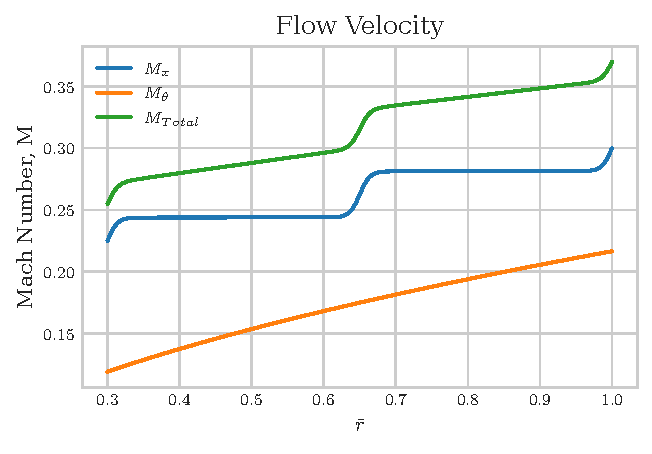
\includegraphics{tex-outputs/MachDistribution.pdf}
%    \caption{Mach distribution for method of manufactured solution case}
%\end{figure}
%
% \begin{figure}
%     \centering
%     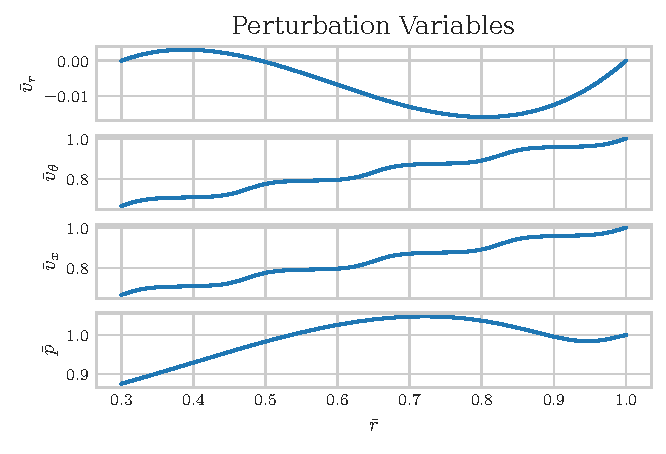
\includegraphics{tex-outputs/PerturbationVariables.pdf}
% \end{figure}
%
% \begin{figure}
%     \centering
%         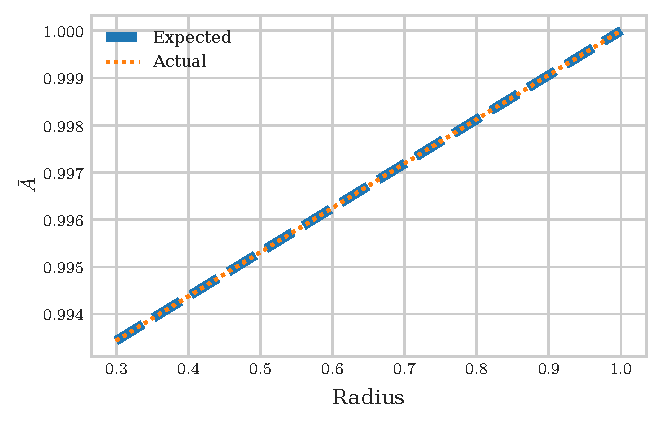
\includegraphics{tex-outputs/SoundSpeedFromIntegration.pdf}
%     \caption{Speed of Sound from Integrating the Tangential Mach Number}
% \end{figure}
%
% \begin{figure}
%     \centering
%         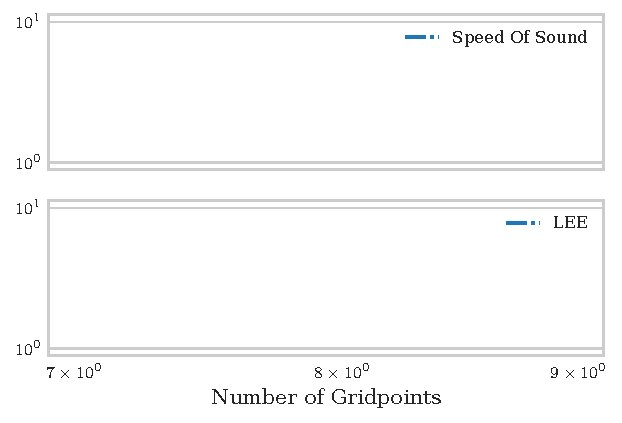
\includegraphics{tex-outputs/L2.pdf}
%     \caption{L2 Norm of the Error for the MMS as a function of Grid Points}
% \end{figure}
%
% \begin{figure}
%     \centering
%         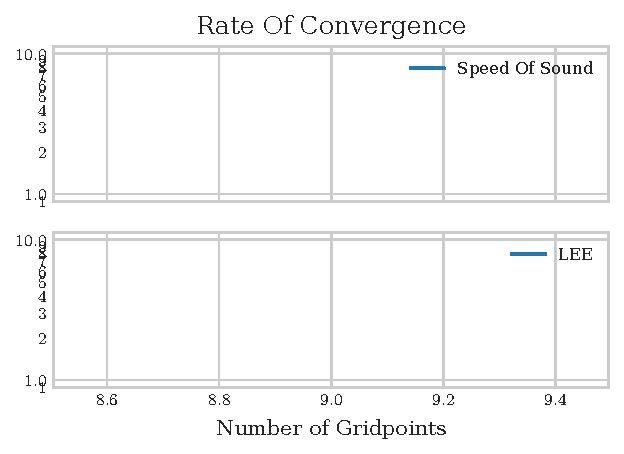
\includegraphics{tex-outputs/ROC.pdf}
%     \caption{Rate of Convergence for the Speed of Sound Integration}
% \end{figure}
%
% \begin{figure}
%         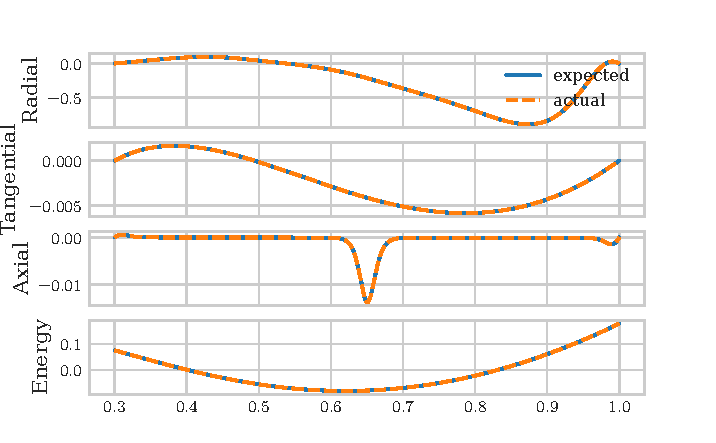
\includegraphics{tex-outputs/SourceTermData.pdf}
%     \caption{Source Term Error}
% \end{figure}
%
% \begin{figure}
%     \centering
%     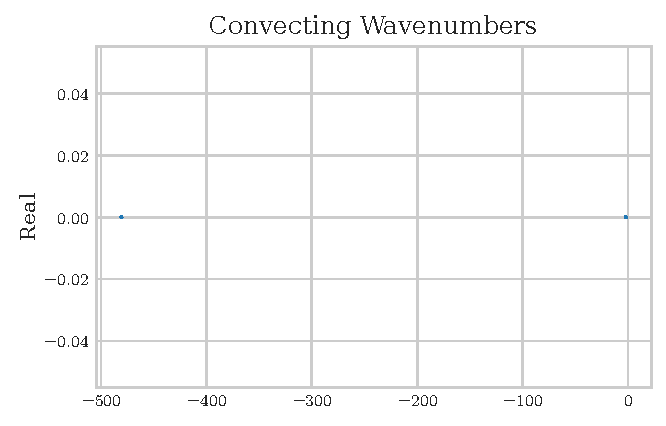
\includegraphics{tex-outputs/cv.waves.scatter.pdf}
% \end{figure}
%%
%\begin{figure}
%    \centering
%    \input{/home/jeff-severino/SWIRL/CodeRun/03-plotReport/tex-outputs/gam.non.acc.0032.tex}
%    \caption{Propagating Modes - 32 Gridpoints}
%\end{figure}
%
%\begin{figure}
%    \centering
%    \small \begin{tabular}{rrrrrr}
\toprule
  \# &   Re\{gam\} &  Im\{gam\} &  Re\{gam/ak\} &  Im\{gam/ak\} &  nz \\
\midrule
106 & -2.000000 &    0.000 &    2.000000 &      -0.000 &  10 \\
 67 &  0.000000 &    0.000 &   -0.000000 &      -0.000 &  10 \\
 16 &  1.301900 &  -32.113 &   -1.301900 &      32.113 &  10 \\
 13 & -0.125380 &  -33.733 &    0.125380 &      33.733 &  11 \\
103 & -2.000000 &    0.000 &    2.000000 &      -0.000 &  11 \\
 43 & -0.092378 &   33.737 &    0.092378 &     -33.737 &  11 \\
 42 &  1.462500 &   33.738 &   -1.462500 &     -33.738 &  11 \\
 14 &  1.429200 &  -33.733 &   -1.429200 &      33.733 &  11 \\
113 & -2.000000 &    0.000 &    2.000000 &      -0.000 &  12 \\
 79 & -2.000000 &    0.000 &    2.000000 &      -0.000 &  12 \\
119 & -2.000000 &    0.000 &    2.000000 &      -0.000 &  12 \\
 68 & -2.000000 &    0.000 &    2.000000 &      -0.000 &  12 \\
115 & -2.000000 &    0.000 &    2.000000 &      -0.000 &  13 \\
114 & -2.000000 &    0.000 &    2.000000 &      -0.000 &  13 \\
 92 & -2.000000 &    0.000 &    2.000000 &      -0.000 &  13 \\
 90 & -2.000000 &    0.000 &    2.000000 &      -0.000 &  13 \\
 85 & -2.000000 &    0.000 &    2.000000 &      -0.000 &  13 \\
 10 & -0.294720 &  -35.725 &    0.294720 &      35.725 &  13 \\
 39 & -0.291950 &   35.723 &    0.291950 &     -35.723 &  13 \\
 38 &  1.628000 &   35.726 &   -1.628000 &     -35.726 &  13 \\
  9 &  1.625800 &  -35.723 &   -1.625800 &      35.723 &  13 \\
  7 & -0.763890 &  -37.070 &    0.763890 &      37.070 &  14 \\
  6 &  0.666670 &   45.864 &   -0.666670 &     -45.864 &  14 \\
 12 &  1.524900 &  -34.972 &   -1.524900 &      34.972 &  14 \\
 96 & -2.000000 &    0.000 &    2.000000 &      -0.000 &  14 \\
 11 & -0.206180 &  -34.972 &    0.206180 &      34.972 &  14 \\
 93 & -2.000000 &    0.000 &    2.000000 &      -0.000 &  14 \\
  2 &  0.666670 &   81.040 &   -0.666670 &     -81.040 &  14 \\
 41 & -0.189800 &   34.974 &    0.189800 &     -34.974 &  14 \\
 82 & -2.000000 &    0.000 &    2.000000 &      -0.000 &  14 \\
 81 & -2.000000 &    0.000 &    2.000000 &      -0.000 &  14 \\
 40 &  1.541200 &   34.974 &   -1.541200 &     -34.974 &  14 \\
 37 & -0.763890 &   37.070 &    0.763890 &     -37.070 &  14 \\
 74 & -2.000000 &    0.000 &    2.000000 &      -0.000 &  14 \\
 36 &  2.097200 &   37.070 &   -2.097200 &     -37.070 &  14 \\
  4 &  0.666670 &  -45.864 &   -0.666670 &      45.864 &  14 \\
 69 & -2.000000 &    0.000 &    2.000000 &      -0.000 &  14 \\
  8 &  2.097200 &  -37.070 &   -2.097200 &      37.070 &  14 \\
  1 &  0.666670 &  -81.040 &   -0.666670 &      81.040 &  14 \\
125 & -2.000000 &    0.000 &    2.000000 &      -0.000 &  15 \\
121 & -2.000000 &    0.000 &    2.000000 &      -0.000 &  15 \\
109 & -2.000000 &    0.000 &    2.000000 &      -0.000 &  15 \\
101 & -2.000000 &    0.000 &    2.000000 &      -0.000 &  15 \\
 97 & -2.000000 &    0.000 &    2.000000 &      -0.000 &  15 \\
 88 & -2.000000 &    0.000 &    2.000000 &      -0.000 &  15 \\
 86 & -2.000000 &    0.000 &    2.000000 &      -0.000 &  15 \\
\bottomrule
\end{tabular}

%    \caption{Propagating Modes - 32 Gridpoints}
%\end{figure}
%
%\begin{figure}
%    \centering
%    \begin{tabular}{rrrrrrr}
\toprule
  \# &          j &   Re\{gam\} &    Im\{gam\} &  Re\{gam/ak\} &  Im\{gam/ak\} &  nz \\
\midrule
256 &  -2.000000 &    0.0000 &   2.000000 &     -0.0000 &           0 & NaN \\
 68 &   0.619830 &   -5.0120 &  -0.619830 &      5.0120 &           1 & NaN \\
128 &   0.410070 &    1.2903 &  -0.410070 &     -1.2903 &           1 & NaN \\
 69 &   0.666670 &   -4.1893 &  -0.666670 &      4.1893 &           1 & NaN \\
 65 &   0.446780 &   -9.1715 &  -0.446780 &      9.1715 &           2 & NaN \\
126 &   1.258500 &    6.0821 &  -1.258500 &     -6.0821 &           2 & NaN \\
 67 &  -5.818700 &   -3.8972 &   5.818700 &      3.8972 &           2 & NaN \\
 63 &   0.456390 &  -13.0120 &  -0.456390 &     13.0120 &           3 & NaN \\
122 &   1.018700 &   13.2630 &  -1.018700 &    -13.2630 &           3 & NaN \\
124 &   1.143500 &    9.6510 &  -1.143500 &     -9.6510 &           3 & NaN \\
 66 &   0.666670 &   -8.2349 &  -0.666670 &      8.2349 &           4 & NaN \\
 61 &   0.482910 &  -16.7060 &  -0.482910 &     16.7060 &           4 & NaN \\
120 &   0.938540 &   16.8600 &  -0.938540 &    -16.8600 &           4 & NaN \\
125 &   0.666660 &    8.2349 &  -0.666660 &     -8.2349 &           5 & NaN \\
 59 &   0.506960 &  -20.3100 &  -0.506960 &     20.3100 &           5 & NaN \\
 60 &   0.667160 &  -19.2820 &  -0.667160 &     19.2820 &           5 & NaN \\
 64 &   0.666720 &  -11.9960 &  -0.666720 &     11.9960 &           5 & NaN \\
123 &   0.666600 &   11.9960 &  -0.666600 &    -11.9960 &           5 & NaN \\
118 &   0.886130 &   20.4130 &  -0.886130 &    -20.4130 &           5 & NaN \\
 55 &   0.526560 &  -23.8360 &  -0.526560 &     23.8360 &           6 & NaN \\
 62 &   0.666860 &  -15.6690 &  -0.666860 &     15.6690 &           6 & NaN \\
116 &   0.849930 &   23.9100 &  -0.849930 &    -23.9100 &           6 & NaN \\
115 &   0.664300 &   26.3400 &  -0.664300 &    -26.3400 &           7 & NaN \\
119 &   0.666060 &   19.2820 &  -0.666060 &    -19.2820 &           7 & NaN \\
 53 &   0.542120 &  -27.2860 &  -0.542120 &     27.2860 &           7 & NaN \\
 54 &   0.668690 &  -26.3410 &  -0.668690 &     26.3410 &           7 & NaN \\
114 &   0.823880 &   27.3420 &  -0.823880 &    -27.3420 &           7 & NaN \\
117 &   0.665410 &   22.8400 &  -0.665410 &    -22.8400 &           8 & NaN \\
127 &   0.666670 &    4.1893 &  -0.666670 &     -4.1893 &           8 & NaN \\
 56 &   0.667720 &  -22.8400 &  -0.667720 &     22.8400 &           8 & NaN \\
121 &   0.666430 &   15.6690 &  -0.666430 &    -15.6690 &           8 & NaN \\
 51 &   0.554190 &  -30.6550 &  -0.554190 &     30.6550 &           8 & NaN \\
112 &   0.804830 &   30.6990 &  -0.804830 &    -30.6990 &           8 & NaN \\
 49 &   0.562870 &  -33.9350 &  -0.562870 &     33.9350 &           9 & NaN \\
110 &   0.791350 &   33.9710 &  -0.791350 &    -33.9710 &           9 & NaN \\
 47 &   0.567160 &  -37.1120 &  -0.567160 &     37.1120 &          10 & NaN \\
113 &   0.662470 &   29.7790 &  -0.662470 &    -29.7790 &          10 & NaN \\
 52 &   0.670330 &  -29.7810 &  -0.670330 &     29.7810 &          10 & NaN \\
 48 &   0.678740 &  -36.4620 &  -0.678740 &     36.4620 &          10 & NaN \\
109 &   0.653460 &   36.4580 &  -0.653460 &    -36.4580 &          10 & NaN \\
108 &   0.783660 &   37.1440 &  -0.783660 &    -37.1440 &          10 & NaN \\
111 &   0.659350 &   33.1530 &  -0.659350 &    -33.1530 &          11 & NaN \\
 50 &   0.673180 &  -33.1550 &  -0.673180 &     33.1550 &          11 & NaN \\
 45 &   0.561210 &  -40.1690 &  -0.561210 &     40.1690 &          11 & NaN \\
 46 &   0.693250 &  -39.7060 &  -0.693250 &     39.7060 &          11 & NaN \\
107 &   0.639090 &   39.6980 &  -0.639090 &    -39.6980 &          11 & NaN \\
106 &   0.786670 &   40.2000 &  -0.786670 &    -40.2000 &          11 & NaN \\
 43 &   0.488190 &  -43.0780 &  -0.488190 &     43.0780 &          12 & NaN \\
 44 &   0.773790 &  -42.8990 &  -0.773790 &     42.8990 &          12 & NaN \\
105 &   0.571750 &   42.8850 &  -0.571750 &    -42.8850 &          12 & NaN \\
104 &   0.844290 &   43.1100 &  -0.844290 &    -43.1100 &          12 & NaN \\
103 &   0.421920 &   45.8950 &  -0.421920 &    -45.8950 &          13 & NaN \\
 41 &   0.344880 &  -45.9680 &  -0.344880 &     45.9680 &          13 & NaN \\
 42 &   0.923820 &  -45.8950 &  -0.923820 &     45.8950 &          13 & NaN \\
102 &   0.985680 &   45.9840 &  -0.985680 &    -45.9840 &          13 & NaN \\
101 &   0.301790 &   48.7410 &  -0.301790 &    -48.7410 &          14 & NaN \\
 40 &   1.040200 &  -48.7380 &  -1.040200 &     48.7380 &          14 & NaN \\
 39 &   0.234520 &  -48.7820 &  -0.234520 &     48.7820 &          14 & NaN \\
100 &   1.098300 &   48.7930 &  -1.098300 &    -48.7930 &          14 & NaN \\
 99 &   0.198080 &   51.4550 &  -0.198080 &    -51.4550 &          15 & NaN \\
 37 &   0.138600 &  -51.4810 &  -0.138600 &     51.4810 &          15 & NaN \\
 38 &   1.141700 &  -51.4520 &  -1.141700 &     51.4520 &          15 & NaN \\
 98 &   1.195300 &   51.4900 &  -1.195300 &    -51.4900 &          15 & NaN \\
 97 &   0.102410 &   54.0370 &  -0.102410 &    -54.0370 &          16 & NaN \\
 36 &   1.235900 &  -54.0340 &  -1.235900 &     54.0340 &          16 & NaN \\
 35 &   0.049547 &  -54.0540 &  -0.049547 &     54.0540 &          16 & NaN \\
 96 &   1.284900 &   54.0610 &  -1.284900 &    -54.0610 &          16 & NaN \\
 94 &   1.370300 &   56.4980 &  -1.370300 &    -56.4980 &          17 & NaN \\
 34 &   1.325900 &  -56.4780 &  -1.325900 &     56.4780 &          17 & NaN \\
 33 &  -0.035624 &  -56.4920 &   0.035624 &     56.4920 &          17 & NaN \\
 95 &   0.011358 &   56.4810 &  -0.011358 &    -56.4810 &          17 & NaN \\
161 &  -2.000000 &    0.0000 &   2.000000 &     -0.0000 &          17 & NaN \\
 93 &  -0.076362 &   58.7810 &   0.076362 &    -58.7810 &          18 & NaN \\
 31 &  -0.117960 &  -58.7880 &   0.117960 &     58.7880 &          18 & NaN \\
 32 &   1.412900 &  -58.7780 &  -1.412900 &     58.7780 &          18 & NaN \\
 92 &   1.452700 &   58.7930 &  -1.452700 &    -58.7930 &          18 & NaN \\
 30 &   1.496700 &  -60.9290 &  -1.496700 &     60.9290 &          19 & NaN \\
 91 &  -0.160810 &   60.9310 &   0.160810 &    -60.9310 &          19 & NaN \\
 90 &   1.532000 &   60.9400 &  -1.532000 &    -60.9400 &          19 & NaN \\
 29 &  -0.197350 &  -60.9360 &   0.197350 &     60.9360 &          19 & NaN \\
170 &  -2.000000 &    0.0000 &   2.000000 &     -0.0000 &          19 & NaN \\
 27 &  -0.272900 &  -62.9290 &   0.272900 &     62.9290 &          20 & NaN \\
 28 &   1.576600 &  -62.9240 &  -1.576600 &     62.9240 &          20 & NaN \\
 89 &  -0.241180 &   62.9260 &   0.241180 &    -62.9260 &          20 & NaN \\
 88 &   1.607400 &   62.9330 &  -1.607400 &    -62.9330 &          20 & NaN \\
135 &  -2.000000 &    0.0000 &   2.000000 &     -0.0000 &          20 & NaN \\
132 &  -2.000000 &    0.0000 &   2.000000 &     -0.0000 &          20 & NaN \\
 26 &   1.651000 &  -64.7590 &  -1.651000 &     64.7590 &          21 & NaN \\
 86 &   1.677500 &   64.7650 &  -1.677500 &    -64.7650 &          21 & NaN \\
 87 &  -0.316040 &   64.7610 &   0.316040 &    -64.7610 &          21 & NaN \\
186 &  -2.000000 &    0.0000 &   2.000000 &     -0.0000 &          21 & NaN \\
 25 &  -0.343080 &  -64.7630 &   0.343080 &     64.7630 &          21 & NaN \\
168 &  -2.000000 &    0.0000 &   2.000000 &     -0.0000 &          21 & NaN \\
164 &  -2.000000 &    0.0000 &   2.000000 &     -0.0000 &          22 & NaN \\
142 &  -2.000000 &    0.0000 &   2.000000 &     -0.0000 &          22 & NaN \\
 24 &  -0.406000 &  -66.4300 &   0.406000 &     66.4300 &          24 & NaN \\
 23 &   1.718200 &  -66.4280 &  -1.718200 &     66.4280 &          24 & NaN \\
 84 &   1.740300 &   66.4320 &  -1.740300 &    -66.4320 &          24 & NaN \\
202 &  -2.000000 &    0.0000 &   2.000000 &     -0.0000 &          24 & NaN \\
 85 &  -0.383500 &   66.4290 &   0.383500 &    -66.4290 &          24 & NaN \\
160 &  -2.000000 &    0.0000 &   2.000000 &     -0.0000 &          24 & NaN \\
155 &  -2.000000 &    0.0000 &   2.000000 &     -0.0000 &          24 & NaN \\
177 &  -2.000000 &    0.0000 &   2.000000 &     -0.0000 &          25 & NaN \\
250 &  -2.000000 &    0.0000 &   2.000000 &     -0.0000 &          26 & NaN \\
159 &  -2.000000 &    0.0000 &   2.000000 &     -0.0000 &          26 & NaN \\
151 &  -2.000000 &    0.0000 &   2.000000 &     -0.0000 &          26 & NaN \\
173 &  -2.000000 &    0.0000 &   2.000000 &     -0.0000 &          26 & NaN \\
238 &  -2.000000 &    0.0000 &   2.000000 &     -0.0000 &          27 & NaN \\
 21 &   1.775700 &  -67.9260 &  -1.775700 &     67.9260 &          27 & NaN \\
204 &  -2.000000 &    0.0000 &   2.000000 &     -0.0000 &          27 & NaN \\
 83 &  -0.441390 &   67.9270 &   0.441390 &    -67.9270 &          27 & NaN \\
 82 &   1.793600 &   67.9290 &  -1.793600 &    -67.9290 &          27 & NaN \\
249 &  -2.000000 &    0.0000 &   2.000000 &     -0.0000 &          27 & NaN \\
 22 &  -0.459500 &  -67.9270 &   0.459500 &     67.9270 &          27 & NaN \\
140 &  -2.000000 &    0.0000 &   2.000000 &     -0.0000 &          27 & NaN \\
255 &  -2.000000 &    0.0000 &   2.000000 &     -0.0000 &          28 & NaN \\
210 &  -2.000000 &    0.0000 &   2.000000 &     -0.0000 &          28 & NaN \\
185 &  -2.000000 &    0.0000 &   2.000000 &     -0.0000 &          28 & NaN \\
183 &  -2.000000 &    0.0000 &   2.000000 &     -0.0000 &          28 & NaN \\
162 &  -2.000000 &    0.0000 &   2.000000 &     -0.0000 &          28 & NaN \\
129 &  -2.000000 &    0.0000 &   2.000000 &     -0.0000 &          28 & NaN \\
  6 &   0.666670 &   93.2360 &  -0.666670 &    -93.2360 &          29 & NaN \\
227 &  -2.000000 &    0.0000 &   2.000000 &     -0.0000 &          29 & NaN \\
196 &  -2.000000 &    0.0000 &   2.000000 &     -0.0000 &          29 & NaN \\
  2 &   0.666670 &  164.7100 &  -0.666670 &   -164.7100 &          29 & NaN \\
180 &  -2.000000 &    0.0000 &   2.000000 &     -0.0000 &          29 & NaN \\
141 &  -2.000000 &    0.0000 &   2.000000 &     -0.0000 &          29 & NaN \\
  3 &   0.666670 &  -93.2360 &  -0.666670 &     93.2360 &          30 & NaN \\
209 &  -2.000000 &    0.0000 &   2.000000 &     -0.0000 &          30 & NaN \\
208 &  -2.000000 &    0.0000 &   2.000000 &     -0.0000 &          30 & NaN \\
 11 &   1.609400 &  -72.5360 &  -1.609400 &     72.5360 &          30 & NaN \\
178 &  -2.000000 &    0.0000 &   2.000000 &     -0.0000 &          30 & NaN \\
244 &  -2.000000 &    0.0000 &   2.000000 &     -0.0000 &          30 & NaN \\
163 &  -2.000000 &    0.0000 &   2.000000 &     -0.0000 &          30 & NaN \\
149 &  -2.000000 &    0.0000 &   2.000000 &     -0.0000 &          30 & NaN \\
 73 &  -0.275930 &   72.5360 &   0.275930 &    -72.5360 &          30 & NaN \\
147 &  -2.000000 &    0.0000 &   2.000000 &     -0.0000 &          30 & NaN \\
 14 &  -0.497270 &  -72.0960 &   0.497270 &     72.0960 &          31 & NaN \\
 58 &  -2.239100 &   75.3730 &   2.239100 &    -75.3730 &          31 & NaN \\
  1 &   0.666670 & -164.7100 &  -0.666670 &    164.7100 &          31 & NaN \\
220 &  -2.000000 &    0.0000 &   2.000000 &     -0.0000 &          31 & NaN \\
218 &  -2.000000 &    0.0000 &   2.000000 &     -0.0000 &          31 & NaN \\
 13 &   1.827400 &  -72.0940 &  -1.827400 &     72.0940 &          31 & NaN \\
200 &  -2.000000 &    0.0000 &   2.000000 &     -0.0000 &          31 & NaN \\
 12 &  -0.276880 &  -72.5380 &   0.276880 &     72.5380 &          31 & NaN \\
176 &  -2.000000 &    0.0000 &   2.000000 &     -0.0000 &          31 & NaN \\
 57 &   3.572500 &   75.3730 &  -3.572500 &    -75.3730 &          31 & NaN \\
 10 &  -1.138600 &  -72.6280 &   1.138600 &     72.6280 &          31 & NaN \\
154 &  -2.000000 &    0.0000 &   2.000000 &     -0.0000 &          31 & NaN \\
 75 &  -0.493770 &   72.0950 &   0.493770 &    -72.0950 &          31 & NaN \\
 74 &   1.830700 &   72.0960 &  -1.830700 &    -72.0960 &          31 & NaN \\
146 &  -2.000000 &    0.0000 &   2.000000 &     -0.0000 &          31 & NaN \\
 72 &   1.610100 &   72.5380 &  -1.610100 &    -72.5380 &          31 & NaN \\
 70 &   2.471900 &   72.6280 &  -2.471900 &    -72.6280 &          31 & NaN \\
  8 &  -2.239100 &  -75.3730 &   2.239100 &     75.3730 &          31 & NaN \\
  7 &   3.572500 &  -75.3730 &  -3.572500 &     75.3730 &          31 & NaN \\
 15 &   1.860800 &  -71.3460 &  -1.860800 &     71.3460 &          32 & NaN \\
235 &  -2.000000 &    0.0000 &   2.000000 &     -0.0000 &          32 & NaN \\
195 &  -2.000000 &    0.0000 &   2.000000 &     -0.0000 &          32 & NaN \\
194 &  -2.000000 &    0.0000 &   2.000000 &     -0.0000 &          32 & NaN \\
188 &  -2.000000 &    0.0000 &   2.000000 &     -0.0000 &          32 & NaN \\
 20 &  -0.501090 &  -69.2490 &   0.501090 &     69.2490 &          32 & NaN \\
 81 &  -0.487170 &   69.2490 &   0.487170 &    -69.2490 &          32 & NaN \\
 80 &   1.835000 &   69.2500 &  -1.835000 &    -69.2500 &          32 & NaN \\
 19 &   1.821300 &  -69.2480 &  -1.821300 &     69.2480 &          32 & NaN \\
174 &  -2.000000 &    0.0000 &   2.000000 &     -0.0000 &          32 & NaN \\
 77 &  -0.527100 &   71.3460 &   0.527100 &    -71.3460 &          32 & NaN \\
 76 &   1.867300 &   71.3470 &  -1.867300 &    -71.3470 &          32 & NaN \\
 71 &  -1.138600 &   72.6280 &   1.138600 &    -72.6280 &          32 & NaN \\
134 &  -2.000000 &    0.0000 &   2.000000 &     -0.0000 &          32 & NaN \\
 16 &  -0.533730 &  -71.3460 &   0.533730 &     71.3460 &          32 & NaN \\
  9 &   2.471900 &  -72.6280 &  -2.471900 &     72.6280 &          32 & NaN \\
252 &  -2.000000 &    0.0000 &   2.000000 &     -0.0000 &          33 & NaN \\
234 &  -2.000000 &    0.0000 &   2.000000 &     -0.0000 &          33 & NaN \\
217 &  -2.000000 &    0.0000 &   2.000000 &     -0.0000 &          33 & NaN \\
215 &  -2.000000 &    0.0000 &   2.000000 &     -0.0000 &          33 & NaN \\
207 &  -2.000000 &    0.0000 &   2.000000 &     -0.0000 &          33 & NaN \\
197 &  -2.000000 &    0.0000 &   2.000000 &     -0.0000 &          33 & NaN \\
193 &  -2.000000 &    0.0000 &   2.000000 &     -0.0000 &          33 & NaN \\
 79 &  -0.517610 &   70.3900 &   0.517610 &    -70.3900 &          33 & NaN \\
 78 &   1.861400 &   70.3910 &  -1.861400 &    -70.3910 &          33 & NaN \\
 18 &  -0.527670 &  -70.3900 &   0.527670 &     70.3900 &          33 & NaN \\
 17 &   1.851500 &  -70.3900 &  -1.851500 &     70.3900 &          33 & NaN \\
189 &  -2.000000 &    0.0000 &   2.000000 &     -0.0000 &          33 & NaN \\
139 &  -2.000000 &    0.0000 &   2.000000 &     -0.0000 &          33 & NaN \\
138 &  -2.000000 &    0.0000 &   2.000000 &     -0.0000 &          33 & NaN \\
137 &  -2.000000 &    0.0000 &   2.000000 &     -0.0000 &          33 & NaN \\
133 &  -2.000000 &    0.0000 &   2.000000 &     -0.0000 &          33 & NaN \\
245 &  -2.000000 &    0.0000 &   2.000000 &     -0.0000 &          34 & NaN \\
236 &  -2.000000 &    0.0000 &   2.000000 &     -0.0000 &          34 & NaN \\
231 &  -2.000000 &    0.0000 &   2.000000 &     -0.0000 &          34 & NaN \\
219 &  -2.000000 &    0.0000 &   2.000000 &     -0.0000 &          34 & NaN \\
167 &  -2.000000 &    0.0000 &   2.000000 &     -0.0000 &          34 & NaN \\
148 &  -2.000000 &    0.0000 &   2.000000 &     -0.0000 &          34 & NaN \\
136 &  -2.000000 &    0.0000 &   2.000000 &     -0.0000 &          34 & NaN \\
221 &  -2.000000 &    0.0000 &   2.000000 &     -0.0000 &          35 & NaN \\
191 &  -2.000000 &    0.0000 &   2.000000 &     -0.0000 &          35 & NaN \\
254 &  -2.000000 &    0.0000 &   2.000000 &     -0.0000 &          36 & NaN \\
201 &  -2.000000 &    0.0000 &   2.000000 &     -0.0000 &          36 & NaN \\
184 &  -2.000000 &    0.0000 &   2.000000 &     -0.0000 &          36 & NaN \\
166 &  -2.000000 &    0.0000 &   2.000000 &     -0.0000 &          36 & NaN \\
223 &  -2.000000 &    0.0000 &   2.000000 &     -0.0000 &          37 & NaN \\
203 &  -2.000000 &    0.0000 &   2.000000 &     -0.0000 &          37 & NaN \\
153 &  -2.000000 &    0.0000 &   2.000000 &     -0.0000 &          37 & NaN \\
143 &  -2.000000 &    0.0000 &   2.000000 &     -0.0000 &          37 & NaN \\
130 &  -2.000000 &    0.0000 &   2.000000 &     -0.0000 &          37 & NaN \\
248 &  -2.000000 &    0.0000 &   2.000000 &     -0.0000 &          38 & NaN \\
224 &  -2.000000 &    0.0000 &   2.000000 &     -0.0000 &          38 & NaN \\
214 &  -2.000000 &    0.0000 &   2.000000 &     -0.0000 &          38 & NaN \\
211 &  -2.000000 &    0.0000 &   2.000000 &     -0.0000 &          38 & NaN \\
187 &  -2.000000 &    0.0000 &   2.000000 &     -0.0000 &          38 & NaN \\
171 &  -2.000000 &    0.0000 &   2.000000 &     -0.0000 &          38 & NaN \\
131 &   0.000000 &    0.0000 &  -0.000000 &     -0.0000 &          38 & NaN \\
247 &  -2.000000 &    0.0000 &   2.000000 &     -0.0000 &          39 & NaN \\
242 &  -2.000000 &    0.0000 &   2.000000 &     -0.0000 &          39 & NaN \\
240 &  -2.000000 &    0.0000 &   2.000000 &     -0.0000 &          39 & NaN \\
226 &  -2.000000 &    0.0000 &   2.000000 &     -0.0000 &          39 & NaN \\
182 &  -2.000000 &    0.0000 &   2.000000 &     -0.0000 &          39 & NaN \\
165 &  -2.000000 &    0.0000 &   2.000000 &     -0.0000 &          39 & NaN \\
152 &  -2.000000 &    0.0000 &   2.000000 &     -0.0000 &          39 & NaN \\
229 &  -2.000000 &    0.0000 &   2.000000 &     -0.0000 &          40 & NaN \\
205 &  -2.000000 &    0.0000 &   2.000000 &     -0.0000 &          40 & NaN \\
150 &  -2.000000 &    0.0000 &   2.000000 &     -0.0000 &          40 & NaN \\
145 &  -2.000000 &    0.0000 &   2.000000 &     -0.0000 &          40 & NaN \\
239 &  -2.000000 &    0.0000 &   2.000000 &     -0.0000 &          41 & NaN \\
233 &  -2.000000 &    0.0000 &   2.000000 &     -0.0000 &          41 & NaN \\
190 &  -2.000000 &    0.0000 &   2.000000 &     -0.0000 &          41 & NaN \\
179 &  -2.000000 &    0.0000 &   2.000000 &     -0.0000 &          41 & NaN \\
156 &  -2.000000 &    0.0000 &   2.000000 &     -0.0000 &          41 & NaN \\
144 &  -2.000000 &    0.0000 &   2.000000 &     -0.0000 &          41 & NaN \\
222 &  -2.000000 &    0.0000 &   2.000000 &     -0.0000 &          42 & NaN \\
172 &  -2.000000 &    0.0000 &   2.000000 &     -0.0000 &          42 & NaN \\
169 &  -2.000000 &    0.0000 &   2.000000 &     -0.0000 &          42 & NaN \\
251 &  -2.000000 &    0.0000 &   2.000000 &     -0.0000 &          43 & NaN \\
192 &  -2.000000 &    0.0000 &   2.000000 &     -0.0000 &          43 & NaN \\
246 &  -2.000000 &    0.0000 &   2.000000 &     -0.0000 &          44 & NaN \\
237 &  -2.000000 &    0.0000 &   2.000000 &     -0.0000 &          44 & NaN \\
198 &  -2.000000 &    0.0000 &   2.000000 &     -0.0000 &          44 & NaN \\
216 &  -2.000000 &    0.0000 &   2.000000 &     -0.0000 &          45 & NaN \\
241 &  -2.000000 &    0.0000 &   2.000000 &     -0.0000 &          46 & NaN \\
225 &  -2.000000 &    0.0000 &   2.000000 &     -0.0000 &          46 & NaN \\
213 &  -2.000000 &    0.0000 &   2.000000 &     -0.0000 &          46 & NaN \\
212 &  -2.000000 &    0.0000 &   2.000000 &     -0.0000 &          46 & NaN \\
206 &  -2.000000 &    0.0000 &   2.000000 &     -0.0000 &          46 & NaN \\
158 &  -2.000000 &    0.0000 &   2.000000 &     -0.0000 &          46 & NaN \\
199 &  -2.000000 &    0.0000 &   2.000000 &     -0.0000 &          47 & NaN \\
175 &  -2.000000 &    0.0000 &   2.000000 &     -0.0000 &          47 & NaN \\
  4 &  82.632000 &    0.0000 & -82.632000 &     -0.0000 &          47 & NaN \\
243 &  -2.000000 &    0.0000 &   2.000000 &     -0.0000 &          48 & NaN \\
230 &  -2.000000 &    0.0000 &   2.000000 &     -0.0000 &          48 & NaN \\
  5 & -81.299000 &    0.0000 &  81.299000 &     -0.0000 &          49 & NaN \\
157 &  -2.000000 &    0.0000 &   2.000000 &     -0.0000 &          49 & NaN \\
228 &  -2.000000 &    0.0000 &   2.000000 &     -0.0000 &          50 & NaN \\
181 &  -2.000000 &    0.0000 &   2.000000 &     -0.0000 &          50 & NaN \\
253 &  -2.000000 &    0.0000 &   2.000000 &     -0.0000 &          56 & NaN \\
232 &  -2.000000 &    0.0000 &   2.000000 &     -0.0000 &          56 & NaN \\
\bottomrule
\end{tabular}

%    \caption{Propagating Modes - 64 Gridpoints}
%\end{figure}
%\begin{figure}
%    \centering
%    \begin{tabular}{rrrrrrr}
\toprule
  \# &           j &   Re\{gam\} &     Im\{gam\} &  Re\{gam/ak\} &  Im\{gam/ak\} &  nz \\
\midrule
512 &   -2.000000 &    0.0000 &    2.000000 &     -0.0000 &           0 & NaN \\
256 &    0.410090 &    1.2904 &   -0.410090 &     -1.2904 &           1 & NaN \\
234 &    0.619610 &   -5.0134 &   -0.619610 &      5.0134 &           1 & NaN \\
235 &    0.666670 &   -4.1716 &   -0.666670 &      4.1716 &           1 & NaN \\
254 &    1.259200 &    6.0844 &   -1.259200 &     -6.0844 &           2 & NaN \\
231 &    0.445680 &   -9.1831 &   -0.445680 &      9.1831 &           2 & NaN \\
233 &   -5.819400 &   -3.8968 &    5.819400 &      3.8968 &           2 & NaN \\
250 &    1.021100 &   13.3030 &   -1.021100 &    -13.3030 &           3 & NaN \\
229 &    0.454500 &  -13.0490 &   -0.454500 &     13.0490 &           3 & NaN \\
252 &    1.145100 &    9.6638 &   -1.145100 &     -9.6638 &           3 & NaN \\
227 &    0.480370 &  -16.7940 &   -0.480370 &     16.7940 &           4 & NaN \\
248 &    0.941490 &   16.9490 &   -0.941490 &    -16.9490 &           4 & NaN \\
223 &    0.503930 &  -20.4770 &   -0.503930 &     20.4770 &           5 & NaN \\
246 &    0.889530 &   20.5820 &   -0.889530 &    -20.5820 &           5 & NaN \\
213 &    0.523280 &  -24.1220 &   -0.523280 &     24.1220 &           6 & NaN \\
244 &    0.853490 &   24.1970 &   -0.853490 &    -24.1970 &           6 & NaN \\
119 &    0.538980 &  -27.7370 &   -0.538980 &     27.7370 &           7 & NaN \\
242 &    0.827190 &   27.7940 &   -0.827190 &    -27.7940 &           7 & NaN \\
117 &    0.551810 &  -31.3260 &   -0.551810 &     31.3260 &           8 & NaN \\
232 &    0.666670 &   -8.2081 &   -0.666670 &      8.2081 &           8 & NaN \\
240 &    0.807210 &   31.3700 &   -0.807210 &    -31.3700 &           8 & NaN \\
115 &    0.562420 &  -34.8890 &   -0.562420 &     34.8890 &           9 & NaN \\
230 &    0.666670 &  -11.9740 &   -0.666670 &     11.9740 &           9 & NaN \\
238 &    0.791560 &   34.9240 &   -0.791560 &    -34.9240 &           9 & NaN \\
113 &    0.571280 &  -38.4250 &   -0.571280 &     38.4250 &          10 & NaN \\
236 &    0.779020 &   38.4540 &   -0.779020 &    -38.4540 &          10 & NaN \\
253 &    0.666670 &    8.2081 &   -0.666670 &     -8.2081 &          11 & NaN \\
111 &    0.578740 &  -41.9340 &   -0.578740 &     41.9340 &          11 & NaN \\
225 &    0.768790 &   41.9590 &   -0.768790 &    -41.9590 &          11 & NaN \\
109 &    0.585060 &  -45.4140 &   -0.585060 &     45.4140 &          12 & NaN \\
228 &    0.666680 &  -15.6700 &   -0.666680 &     15.6700 &          12 & NaN \\
221 &    0.760350 &   45.4350 &   -0.760350 &    -45.4350 &          12 & NaN \\
107 &    0.590400 &  -48.8630 &   -0.590400 &     48.8630 &          13 & NaN \\
251 &    0.666660 &   11.9740 &   -0.666660 &    -11.9740 &          13 & NaN \\
219 &    0.753350 &   48.8810 &   -0.753350 &    -48.8810 &          13 & NaN \\
118 &    0.666910 &  -30.1860 &   -0.666910 &     30.1860 &          14 & NaN \\
255 &    0.666670 &    4.1716 &   -0.666670 &     -4.1716 &          14 & NaN \\
241 &    0.666380 &   30.1860 &   -0.666380 &    -30.1860 &          14 & NaN \\
105 &    0.594870 &  -52.2790 &   -0.594870 &     52.2790 &          14 & NaN \\
249 &    0.666650 &   15.6700 &   -0.666650 &    -15.6700 &          14 & NaN \\
217 &    0.747560 &   52.2940 &   -0.747560 &    -52.2940 &          14 & NaN \\
243 &    0.666490 &   26.5880 &   -0.666490 &    -26.5880 &          15 & NaN \\
103 &    0.598540 &  -55.6580 &   -0.598540 &     55.6580 &          15 & NaN \\
104 &    0.669930 &  -54.7430 &   -0.669930 &     54.7430 &          15 & NaN \\
216 &    0.663090 &   54.7430 &   -0.663090 &    -54.7430 &          15 & NaN \\
120 &    0.666810 &  -26.5880 &   -0.666810 &     26.5880 &          15 & NaN \\
224 &    0.666700 &  -19.3320 &   -0.666700 &     19.3320 &          15 & NaN \\
215 &    0.742840 &   55.6720 &   -0.742840 &    -55.6720 &          15 & NaN \\
245 &    0.666570 &   22.9700 &   -0.666570 &    -22.9700 &          16 & NaN \\
101 &    0.601370 &  -58.9990 &   -0.601370 &     58.9990 &          16 & NaN \\
214 &    0.666740 &  -22.9700 &   -0.666740 &     22.9700 &          16 & NaN \\
211 &    0.739170 &   59.0120 &   -0.739170 &    -59.0120 &          16 & NaN \\
247 &    0.666620 &   19.3320 &   -0.666620 &    -19.3320 &          17 & NaN \\
239 &    0.666220 &   33.7640 &   -0.666220 &    -33.7640 &          17 & NaN \\
 99 &    0.603230 &  -62.2980 &   -0.603230 &     62.2980 &          17 & NaN \\
116 &    0.667050 &  -33.7640 &   -0.667050 &     33.7640 &          17 & NaN \\
209 &    0.736650 &   62.3100 &   -0.736650 &    -62.3100 &          17 & NaN \\
222 &    0.665300 &   44.3670 &   -0.665300 &    -44.3670 &          18 & NaN \\
 97 &    0.603730 &  -65.5510 &   -0.603730 &     65.5510 &          18 & NaN \\
110 &    0.667890 &  -44.3670 &   -0.667890 &     44.3670 &          18 & NaN \\
207 &    0.735650 &   65.5620 &   -0.735650 &    -65.5620 &          18 & NaN \\
 95 &    0.601730 &  -68.7520 &   -0.601730 &     68.7520 &          19 & NaN \\
220 &    0.664760 &   47.8520 &   -0.664760 &    -47.8520 &          19 & NaN \\
108 &    0.668380 &  -47.8530 &   -0.668380 &     47.8530 &          19 & NaN \\
205 &    0.737290 &   68.7630 &   -0.737290 &    -68.7630 &          19 & NaN \\
218 &    0.664050 &   51.3120 &   -0.664050 &    -51.3120 &          20 & NaN \\
 93 &    0.592640 &  -71.8900 &   -0.592640 &     71.8900 &          20 & NaN \\
106 &    0.669040 &  -51.3120 &   -0.669040 &     51.3120 &          20 & NaN \\
203 &    0.745940 &   71.9010 &   -0.745940 &    -71.9010 &          20 & NaN \\
112 &    0.667520 &  -40.8560 &   -0.667520 &     40.8560 &          21 & NaN \\
226 &    0.665700 &   40.8560 &   -0.665700 &    -40.8560 &          21 & NaN \\
202 &    0.587570 &   74.7580 &   -0.587570 &    -74.7580 &          21 & NaN \\
210 &    0.659830 &   61.5180 &   -0.659830 &    -61.5180 &          21 & NaN \\
100 &    0.672990 &  -61.5190 &   -0.672990 &     61.5190 &          21 & NaN \\
 92 &    0.750460 &  -74.7660 &   -0.750460 &     74.7660 &          21 & NaN \\
 91 &    0.537490 &  -74.9450 &   -0.537490 &     74.9450 &          21 & NaN \\
201 &    0.795100 &   74.9590 &   -0.795100 &    -74.9590 &          21 & NaN \\
212 &    0.661760 &   58.1450 &   -0.661760 &    -58.1450 &          22 & NaN \\
 89 &    0.415940 &  -78.0210 &   -0.415940 &     78.0210 &          22 & NaN \\
200 &    0.465230 &   77.9440 &   -0.465230 &    -77.9440 &          22 & NaN \\
102 &    0.671180 &  -58.1460 &   -0.671180 &     58.1460 &          22 & NaN \\
208 &    0.656850 &   64.8610 &   -0.656850 &    -64.8610 &          22 & NaN \\
 90 &    0.874380 &  -77.9450 &   -0.874380 &     77.9450 &          22 & NaN \\
237 &    0.666000 &   37.3210 &   -0.666000 &    -37.3210 &          22 & NaN \\
114 &    0.667250 &  -37.3210 &   -0.667250 &     37.3210 &          22 & NaN \\
 98 &    0.675830 &  -64.8620 &   -0.675830 &     64.8620 &          22 & NaN \\
199 &    0.914710 &   78.0280 &   -0.914710 &    -78.0280 &          22 & NaN \\
263 &   -2.000000 &    0.0000 &    2.000000 &     -0.0000 &          22 & NaN \\
198 &    0.370230 &   81.0390 &   -0.370230 &    -81.0390 &          23 & NaN \\
206 &    0.651620 &   68.1760 &   -0.651620 &    -68.1760 &          23 & NaN \\
 87 &    0.324710 &  -81.0880 &   -0.324710 &     81.0880 &          23 & NaN \\
 96 &    0.680870 &  -68.1780 &   -0.680870 &     68.1780 &          23 & NaN \\
 88 &    0.967820 &  -81.0380 &   -0.967820 &     81.0380 &          23 & NaN \\
197 &    1.007200 &   81.0930 &   -1.007200 &    -81.0930 &          23 & NaN \\
196 &    0.291170 &   84.0760 &   -0.291170 &    -84.0760 &          24 & NaN \\
 86 &    1.045900 &  -84.0750 &   -1.045900 &     84.0750 &          24 & NaN \\
 85 &    0.248680 &  -84.1120 &   -0.248680 &     84.1120 &          24 & NaN \\
195 &    1.083900 &   84.1160 &   -1.083900 &    -84.1160 &          24 & NaN \\
 83 &    0.180560 &  -87.0870 &   -0.180560 &     87.0870 &          25 & NaN \\
 84 &    1.116000 &  -87.0590 &   -1.116000 &     87.0590 &          25 & NaN \\
194 &    0.220470 &   87.0600 &   -0.220470 &    -87.0600 &          25 & NaN \\
193 &    1.152400 &   87.0910 &   -1.152400 &    -87.0910 &          25 & NaN \\
 81 &    0.117260 &  -90.0110 &   -0.117260 &     90.0110 &          26 & NaN \\
 94 &    0.692740 &  -71.4750 &   -0.692740 &     71.4750 &          26 & NaN \\
204 &    0.639710 &   71.4700 &   -0.639710 &    -71.4700 &          26 & NaN \\
192 &    0.154880 &   89.9890 &   -0.154880 &    -89.9890 &          26 & NaN \\
 82 &    1.181100 &  -89.9880 &   -1.181100 &     89.9880 &          26 & NaN \\
191 &    1.216000 &   90.0140 &   -1.216000 &    -90.0140 &          26 & NaN \\
190 &    0.092723 &   92.8620 &   -0.092723 &    -92.8620 &          27 & NaN \\
 79 &    0.057178 &  -92.8800 &   -0.057178 &     92.8800 &          27 & NaN \\
 80 &    1.242900 &  -92.8610 &   -1.242900 &     92.8610 &          27 & NaN \\
189 &    1.276200 &   92.8830 &   -1.276200 &    -92.8830 &          27 & NaN \\
188 &    0.033037 &   95.6780 &   -0.033037 &    -95.6780 &          28 & NaN \\
 78 &    1.302300 &  -95.6770 &   -1.302300 &     95.6770 &          28 & NaN \\
 77 &    0.000000 &  -95.6930 &   -0.000000 &     95.6930 &          28 & NaN \\
187 &    1.334100 &   95.6960 &   -1.334100 &    -95.6960 &          28 & NaN \\
185 &    1.390200 &   98.4500 &   -1.390200 &    -98.4500 &          29 & NaN \\
 76 &    1.359800 &  -98.4340 &   -1.359800 &     98.4340 &          29 & NaN \\
 75 &   -0.056616 &  -98.4480 &    0.056616 &     98.4480 &          29 & NaN \\
186 &   -0.024755 &   98.4350 &    0.024755 &    -98.4350 &          29 & NaN \\
183 &    1.444800 &  101.1400 &   -1.444800 &   -101.1400 &          30 & NaN \\
 74 &    1.415900 & -101.1300 &   -1.415900 &    101.1300 &          30 & NaN \\
184 &   -0.081013 &  101.1300 &    0.081013 &   -101.1300 &          30 & NaN \\
 73 &   -0.111210 & -101.1400 &    0.111210 &    101.1400 &          30 & NaN \\
 71 &   -0.164580 & -103.7800 &    0.164580 &    103.7800 &          31 & NaN \\
431 &   -2.000000 &    0.0000 &    2.000000 &     -0.0000 &          31 & NaN \\
181 &    1.498200 &  103.7800 &   -1.498200 &   -103.7800 &          31 & NaN \\
182 &   -0.135950 &  103.7700 &    0.135950 &   -103.7700 &          31 & NaN \\
 72 &    1.470700 & -103.7700 &   -1.470700 &    103.7700 &          31 & NaN \\
 70 &    1.524300 & -106.3400 &   -1.524300 &    106.3400 &          32 & NaN \\
179 &    1.550500 &  106.3500 &   -1.550500 &   -106.3500 &          32 & NaN \\
180 &   -0.189690 &  106.3400 &    0.189690 &   -106.3400 &          32 & NaN \\
 69 &   -0.216820 & -106.3500 &    0.216820 &    106.3500 &          32 & NaN \\
178 &   -0.242260 &  108.8400 &    0.242260 &   -108.8400 &          33 & NaN \\
177 &    1.601700 &  108.8500 &   -1.601700 &   -108.8500 &          33 & NaN \\
 68 &    1.576700 & -108.8400 &   -1.576700 &    108.8400 &          33 & NaN \\
 67 &   -0.267980 & -108.8500 &    0.267980 &    108.8500 &          33 & NaN \\
176 &   -0.293680 &  111.2800 &    0.293680 &   -111.2800 &          34 & NaN \\
175 &    1.651700 &  111.2900 &   -1.651700 &   -111.2900 &          34 & NaN \\
 66 &    1.628000 & -111.2800 &   -1.628000 &    111.2800 &          34 & NaN \\
 65 &   -0.318020 & -111.2900 &    0.318020 &    111.2900 &          34 & NaN \\
 63 &   -0.366900 & -113.6600 &    0.366900 &    113.6600 &          35 & NaN \\
173 &    1.700600 &  113.6600 &   -1.700600 &   -113.6600 &          35 & NaN \\
174 &   -0.343870 &  113.6500 &    0.343870 &   -113.6500 &          35 & NaN \\
 64 &    1.678100 & -113.6500 &   -1.678100 &    113.6500 &          35 & NaN \\
 60 &    1.774400 & -118.1800 &   -1.774400 &    118.1800 &          37 & NaN \\
169 &    1.794400 &  118.1800 &   -1.794400 &   -118.1800 &          37 & NaN \\
 59 &   -0.460790 & -118.1800 &    0.460790 &    118.1800 &          37 & NaN \\
170 &   -0.440280 &  118.1800 &    0.440280 &   -118.1800 &          37 & NaN \\
262 &   -2.000000 &    0.0000 &    2.000000 &     -0.0000 &          37 & NaN \\
 62 &    1.727000 & -115.9500 &   -1.727000 &    115.9500 &          38 & NaN \\
 61 &   -0.414530 & -115.9600 &    0.414530 &    115.9600 &          38 & NaN \\
172 &   -0.392770 &  115.9500 &    0.392770 &   -115.9500 &          38 & NaN \\
171 &    1.748200 &  115.9600 &   -1.748200 &   -115.9600 &          38 & NaN \\
347 &   -2.000000 &    0.0000 &    2.000000 &     -0.0000 &          39 & NaN \\
282 &   -2.000000 &    0.0000 &    2.000000 &     -0.0000 &          39 & NaN \\
 52 &    1.947400 & -126.3500 &   -1.947400 &    126.3500 &          41 & NaN \\
 51 &   -0.629410 & -126.3500 &    0.629410 &    126.3500 &          41 & NaN \\
161 &    1.963000 &  126.3500 &   -1.963000 &   -126.3500 &          41 & NaN \\
321 &   -2.000000 &    0.0000 &    2.000000 &     -0.0000 &          41 & NaN \\
162 &   -0.613580 &  126.3500 &    0.613580 &   -126.3500 &          41 & NaN \\
 57 &   -0.505560 & -120.3400 &    0.505560 &    120.3400 &          42 & NaN \\
167 &    1.839200 &  120.3400 &   -1.839200 &   -120.3400 &          42 & NaN \\
403 &   -2.000000 &    0.0000 &    2.000000 &     -0.0000 &          42 & NaN \\
 58 &    1.820300 & -120.3300 &   -1.820300 &    120.3300 &          42 & NaN \\
349 &   -2.000000 &    0.0000 &    2.000000 &     -0.0000 &          42 & NaN \\
294 &   -2.000000 &    0.0000 &    2.000000 &     -0.0000 &          42 & NaN \\
168 &   -0.486250 &  120.3300 &    0.486250 &   -120.3300 &          42 & NaN \\
 56 &    1.864500 & -122.4200 &   -1.864500 &    122.4200 &          43 & NaN \\
 55 &   -0.548690 & -122.4200 &    0.548690 &    122.4200 &          43 & NaN \\
166 &   -0.530560 &  122.4200 &    0.530560 &   -122.4200 &          43 & NaN \\
501 &   -2.000000 &    0.0000 &    2.000000 &     -0.0000 &          43 & NaN \\
165 &    1.882300 &  122.4200 &   -1.882300 &   -122.4200 &          43 & NaN \\
305 &   -2.000000 &    0.0000 &    2.000000 &     -0.0000 &          43 & NaN \\
394 &   -2.000000 &    0.0000 &    2.000000 &     -0.0000 &          43 & NaN \\
258 &   -2.000000 &    0.0000 &    2.000000 &     -0.0000 &          43 & NaN \\
415 &   -2.000000 &    0.0000 &    2.000000 &     -0.0000 &          44 & NaN \\
374 &   -2.000000 &    0.0000 &    2.000000 &     -0.0000 &          44 & NaN \\
319 &   -2.000000 &    0.0000 &    2.000000 &     -0.0000 &          44 & NaN \\
337 &   -2.000000 &    0.0000 &    2.000000 &     -0.0000 &          44 & NaN \\
280 &   -2.000000 &    0.0000 &    2.000000 &     -0.0000 &          44 & NaN \\
276 &   -2.000000 &    0.0000 &    2.000000 &     -0.0000 &          44 & NaN \\
272 &   -2.000000 &    0.0000 &    2.000000 &     -0.0000 &          44 & NaN \\
297 &   -2.000000 &    0.0000 &    2.000000 &     -0.0000 &          45 & NaN \\
376 &   -2.000000 &    0.0000 &    2.000000 &     -0.0000 &          46 & NaN \\
351 &   -2.000000 &    0.0000 &    2.000000 &     -0.0000 &          46 & NaN \\
332 &   -2.000000 &    0.0000 &    2.000000 &     -0.0000 &          46 & NaN \\
271 &   -2.000000 &    0.0000 &    2.000000 &     -0.0000 &          46 & NaN \\
437 &   -2.000000 &    0.0000 &    2.000000 &     -0.0000 &          47 & NaN \\
324 &   -2.000000 &    0.0000 &    2.000000 &     -0.0000 &          47 & NaN \\
339 &   -2.000000 &    0.0000 &    2.000000 &     -0.0000 &          47 & NaN \\
299 &   -2.000000 &    0.0000 &    2.000000 &     -0.0000 &          47 & NaN \\
296 &   -2.000000 &    0.0000 &    2.000000 &     -0.0000 &          47 & NaN \\
441 &   -2.000000 &    0.0000 &    2.000000 &     -0.0000 &          48 & NaN \\
382 &   -2.000000 &    0.0000 &    2.000000 &     -0.0000 &          48 & NaN \\
335 &   -2.000000 &    0.0000 &    2.000000 &     -0.0000 &          48 & NaN \\
310 &   -2.000000 &    0.0000 &    2.000000 &     -0.0000 &          48 & NaN \\
359 &   -2.000000 &    0.0000 &    2.000000 &     -0.0000 &          49 & NaN \\
357 &   -2.000000 &    0.0000 &    2.000000 &     -0.0000 &          49 & NaN \\
342 &   -2.000000 &    0.0000 &    2.000000 &     -0.0000 &          49 & NaN \\
274 &   -2.000000 &    0.0000 &    2.000000 &     -0.0000 &          49 & NaN \\
 53 &   -0.590030 & -124.4300 &    0.590030 &    124.4300 &          50 & NaN \\
 54 &    1.907000 & -124.4200 &   -1.907000 &    124.4200 &          50 & NaN \\
373 &   -2.000000 &    0.0000 &    2.000000 &     -0.0000 &          50 & NaN \\
164 &   -0.573060 &  124.4200 &    0.573060 &   -124.4200 &          50 & NaN \\
163 &    1.923600 &  124.4300 &   -1.923600 &   -124.4300 &          50 & NaN \\
300 &   -2.000000 &    0.0000 &    2.000000 &     -0.0000 &          50 & NaN \\
298 &   -2.000000 &    0.0000 &    2.000000 &     -0.0000 &          50 & NaN \\
323 &   -2.000000 &    0.0000 &    2.000000 &     -0.0000 &          51 & NaN \\
375 &   -2.000000 &    0.0000 &    2.000000 &     -0.0000 &          52 & NaN \\
344 &   -2.000000 &    0.0000 &    2.000000 &     -0.0000 &          52 & NaN \\
286 &   -2.000000 &    0.0000 &    2.000000 &     -0.0000 &          52 & NaN \\
325 &   -2.000000 &    0.0000 &    2.000000 &     -0.0000 &          53 & NaN \\
289 &   -2.000000 &    0.0000 &    2.000000 &     -0.0000 &          53 & NaN \\
420 &   -2.000000 &    0.0000 &    2.000000 &     -0.0000 &          54 & NaN \\
 50 &    1.985800 & -128.2000 &   -1.985800 &    128.2000 &          54 & NaN \\
 49 &   -0.666670 & -128.2000 &    0.666670 &    128.2000 &          54 & NaN \\
159 &    2.000300 &  128.2000 &   -2.000300 &   -128.2000 &          54 & NaN \\
160 &   -0.651950 &  128.2000 &    0.651950 &   -128.2000 &          54 & NaN \\
312 &   -2.000000 &    0.0000 &    2.000000 &     -0.0000 &          54 & NaN \\
301 &   -2.000000 &    0.0000 &    2.000000 &     -0.0000 &          54 & NaN \\
266 &   -2.000000 &    0.0000 &    2.000000 &     -0.0000 &          54 & NaN \\
260 &   -2.000000 &    0.0000 &    2.000000 &     -0.0000 &          54 & NaN \\
419 &   -2.000000 &    0.0000 &    2.000000 &     -0.0000 &          55 & NaN \\
396 &   -2.000000 &    0.0000 &    2.000000 &     -0.0000 &          55 & NaN \\
361 &   -2.000000 &    0.0000 &    2.000000 &     -0.0000 &          55 & NaN \\
311 &   -2.000000 &    0.0000 &    2.000000 &     -0.0000 &          55 & NaN \\
268 &   -2.000000 &    0.0000 &    2.000000 &     -0.0000 &          55 & NaN \\
428 &   -2.000000 &    0.0000 &    2.000000 &     -0.0000 &          56 & NaN \\
414 &   -2.000000 &    0.0000 &    2.000000 &     -0.0000 &          56 & NaN \\
389 &   -2.000000 &    0.0000 &    2.000000 &     -0.0000 &          56 & NaN \\
485 &   -2.000000 &    0.0000 &    2.000000 &     -0.0000 &          57 & NaN \\
498 &   -2.000000 &    0.0000 &    2.000000 &     -0.0000 &          57 & NaN \\
468 &   -2.000000 &    0.0000 &    2.000000 &     -0.0000 &          57 & NaN \\
448 &   -2.000000 &    0.0000 &    2.000000 &     -0.0000 &          57 & NaN \\
427 &   -2.000000 &    0.0000 &    2.000000 &     -0.0000 &          57 & NaN \\
380 &   -2.000000 &    0.0000 &    2.000000 &     -0.0000 &          57 & NaN \\
290 &   -2.000000 &    0.0000 &    2.000000 &     -0.0000 &          57 & NaN \\
366 &   -2.000000 &    0.0000 &    2.000000 &     -0.0000 &          58 & NaN \\
478 &   -2.000000 &    0.0000 &    2.000000 &     -0.0000 &          58 & NaN \\
454 &   -2.000000 &    0.0000 &    2.000000 &     -0.0000 &          58 & NaN \\
423 &   -2.000000 &    0.0000 &    2.000000 &     -0.0000 &          58 & NaN \\
355 &   -2.000000 &    0.0000 &    2.000000 &     -0.0000 &          58 & NaN \\
333 &   -2.000000 &    0.0000 &    2.000000 &     -0.0000 &          58 & NaN \\
318 &   -2.000000 &    0.0000 &    2.000000 &     -0.0000 &          58 & NaN \\
306 &   -2.000000 &    0.0000 &    2.000000 &     -0.0000 &          58 & NaN \\
303 &   -2.000000 &    0.0000 &    2.000000 &     -0.0000 &          58 & NaN \\
341 &   -2.000000 &    0.0000 &    2.000000 &     -0.0000 &          59 & NaN \\
308 &   -2.000000 &    0.0000 &    2.000000 &     -0.0000 &          59 & NaN \\
489 &   -2.000000 &    0.0000 &    2.000000 &     -0.0000 &          60 & NaN \\
378 &   -2.000000 &    0.0000 &    2.000000 &     -0.0000 &          60 & NaN \\
348 &   -2.000000 &    0.0000 &    2.000000 &     -0.0000 &          60 & NaN \\
336 &   -2.000000 &    0.0000 &    2.000000 &     -0.0000 &          60 & NaN \\
459 &   -2.000000 &    0.0000 &    2.000000 &     -0.0000 &          61 & NaN \\
410 &   -2.000000 &    0.0000 &    2.000000 &     -0.0000 &          61 & NaN \\
409 &   -2.000000 &    0.0000 &    2.000000 &     -0.0000 &          61 & NaN \\
494 &   -2.000000 &    0.0000 &    2.000000 &     -0.0000 &          61 & NaN \\
365 &   -2.000000 &    0.0000 &    2.000000 &     -0.0000 &          61 & NaN \\
354 &   -2.000000 &    0.0000 &    2.000000 &     -0.0000 &          61 & NaN \\
433 &   -2.000000 &    0.0000 &    2.000000 &     -0.0000 &          61 & NaN \\
275 &   -2.000000 &    0.0000 &    2.000000 &     -0.0000 &          61 & NaN \\
259 &    0.000000 &    0.0000 &   -0.000000 &     -0.0000 &          61 & NaN \\
  1 &    0.666670 & -332.0500 &   -0.666670 &    332.0500 &          62 & NaN \\
320 &   -2.000000 &    0.0000 &    2.000000 &     -0.0000 &          62 & NaN \\
295 &   -2.000000 &    0.0000 &    2.000000 &     -0.0000 &          62 & NaN \\
456 &   -2.000000 &    0.0000 &    2.000000 &     -0.0000 &          63 & NaN \\
432 &   -2.000000 &    0.0000 &    2.000000 &     -0.0000 &          63 & NaN \\
422 &   -2.000000 &    0.0000 &    2.000000 &     -0.0000 &          63 & NaN \\
418 &   -2.000000 &    0.0000 &    2.000000 &     -0.0000 &          63 & NaN \\
  3 &    0.666670 & -187.9700 &   -0.666670 &    187.9700 &          63 & NaN \\
391 &   -2.000000 &    0.0000 &    2.000000 &     -0.0000 &          63 & NaN \\
 48 &    2.021800 & -129.9700 &   -2.021800 &    129.9700 &          63 & NaN \\
  2 &    0.666670 &  332.0500 &   -0.666670 &   -332.0500 &          63 & NaN \\
 47 &   -0.701620 & -129.9800 &    0.701620 &    129.9800 &          63 & NaN \\
327 &   -2.000000 &    0.0000 &    2.000000 &     -0.0000 &          63 & NaN \\
158 &   -0.688010 &  129.9700 &    0.688010 &   -129.9700 &          63 & NaN \\
157 &    2.035200 &  129.9800 &   -2.035200 &   -129.9800 &          63 & NaN \\
264 &   -2.000000 &    0.0000 &    2.000000 &     -0.0000 &          63 & NaN \\
125 &   -0.436750 &  146.2200 &    0.436750 &   -146.2200 &          64 & NaN \\
127 &    1.517800 &  146.4800 &   -1.517800 &   -146.4800 &          64 & NaN \\
 15 &    1.770100 & -146.2200 &   -1.770100 &    146.2200 &          64 & NaN \\
472 &   -2.000000 &    0.0000 &    2.000000 &     -0.0000 &          64 & NaN \\
446 &   -2.000000 &    0.0000 &    2.000000 &     -0.0000 &          64 & NaN \\
  6 &    0.666670 &  187.9700 &   -0.666670 &   -187.9700 &          64 & NaN \\
369 &   -2.000000 &    0.0000 &    2.000000 &     -0.0000 &          64 & NaN \\
 46 &    2.055300 & -131.6600 &   -2.055300 &    131.6600 &          64 & NaN \\
 45 &   -0.734080 & -131.6700 &    0.734080 &    131.6700 &          64 & NaN \\
328 &   -2.000000 &    0.0000 &    2.000000 &     -0.0000 &          64 & NaN \\
326 &   -2.000000 &    0.0000 &    2.000000 &     -0.0000 &          64 & NaN \\
156 &   -0.721550 &  131.6600 &    0.721550 &   -131.6600 &          64 & NaN \\
155 &    2.067600 &  131.6700 &   -2.067600 &   -131.6700 &          64 & NaN \\
 18 &   -0.437220 & -146.2200 &    0.437220 &    146.2200 &          64 & NaN \\
 17 &   -0.184480 & -146.4800 &    0.184480 &    146.4800 &          64 & NaN \\
128 &    1.770500 &  146.2200 &   -1.770500 &   -146.2200 &          64 & NaN \\
126 &   -0.663690 &  145.8800 &    0.663690 &   -145.8800 &          65 & NaN \\
 14 &    2.410700 & -145.7200 &   -2.410700 &    145.7200 &          65 & NaN \\
124 &   -1.077400 &  145.7200 &    1.077400 &   -145.7200 &          65 & NaN \\
123 &   -0.184250 &  146.4700 &    0.184250 &   -146.4700 &          65 & NaN \\
 13 &    1.517600 & -146.4700 &   -1.517600 &    146.4700 &          65 & NaN \\
404 &   -2.000000 &    0.0000 &    2.000000 &     -0.0000 &          65 & NaN \\
 20 &   -0.664600 & -145.8800 &    0.664600 &    145.8800 &          65 & NaN \\
 40 &    2.138700 & -136.2400 &   -2.138700 &    136.2400 &          65 & NaN \\
 39 &   -0.814430 & -136.2400 &    0.814430 &    136.2400 &          65 & NaN \\
309 &   -2.000000 &    0.0000 &    2.000000 &     -0.0000 &          65 & NaN \\
149 &    2.147900 &  136.2400 &   -2.147900 &   -136.2400 &          65 & NaN \\
273 &   -2.000000 &    0.0000 &    2.000000 &     -0.0000 &          65 & NaN \\
269 &   -2.000000 &    0.0000 &    2.000000 &     -0.0000 &          65 & NaN \\
 16 &    1.997100 & -145.8800 &   -1.997100 &    145.8800 &          65 & NaN \\
130 &    1.997900 &  145.8800 &   -1.997900 &   -145.8800 &          65 & NaN \\
122 &    4.305600 &  146.4300 &   -4.305600 &   -146.4300 &          66 & NaN \\
  7 &   -5.190400 & -151.9600 &    5.190400 &    151.9600 &          66 & NaN \\
398 &   -2.000000 &    0.0000 &    2.000000 &     -0.0000 &          66 & NaN \\
 12 &   -2.972300 & -146.4300 &    2.972300 &    146.4300 &          66 & NaN \\
 22 &   -0.816460 & -145.3000 &    0.816460 &    145.3000 &          66 & NaN \\
362 &   -2.000000 &    0.0000 &    2.000000 &     -0.0000 &          66 & NaN \\
360 &   -2.000000 &    0.0000 &    2.000000 &     -0.0000 &          66 & NaN \\
 21 &    2.148000 & -145.3000 &   -2.148000 &    145.3000 &          66 & NaN \\
 42 &    2.113900 & -134.8000 &   -2.113900 &    134.8000 &          66 & NaN \\
 10 &    6.523700 &  151.9600 &   -6.523700 &   -151.9600 &          66 & NaN \\
 41 &   -0.790710 & -134.8000 &    0.790710 &    134.8000 &          66 & NaN \\
152 &   -0.780300 &  134.8000 &    0.780300 &   -134.8000 &          66 & NaN \\
 19 &   -1.077400 & -145.7200 &    1.077400 &    145.7200 &          66 & NaN \\
151 &    2.124200 &  134.8000 &   -2.124200 &   -134.8000 &          66 & NaN \\
293 &   -2.000000 &    0.0000 &    2.000000 &     -0.0000 &          66 & NaN \\
291 &   -2.000000 &    0.0000 &    2.000000 &     -0.0000 &          66 & NaN \\
132 &    2.149800 &  145.3000 &   -2.149800 &   -145.3000 &          66 & NaN \\
131 &   -0.814610 &  145.3000 &    0.814610 &   -145.3000 &          66 & NaN \\
129 &    2.410800 &  145.7200 &   -2.410800 &   -145.7200 &          66 & NaN \\
121 &   -2.972300 &  146.4300 &    2.972300 &   -146.4300 &          67 & NaN \\
450 &   -2.000000 &    0.0000 &    2.000000 &     -0.0000 &          67 & NaN \\
444 &   -2.000000 &    0.0000 &    2.000000 &     -0.0000 &          67 & NaN \\
436 &   -2.000000 &    0.0000 &    2.000000 &     -0.0000 &          67 & NaN \\
 24 &   -0.842410 & -144.6400 &    0.842410 &    144.6400 &          67 & NaN \\
387 &   -2.000000 &    0.0000 &    2.000000 &     -0.0000 &          67 & NaN \\
 23 &    2.173400 & -144.6400 &   -2.173400 &    144.6400 &          67 & NaN \\
 44 &    2.086100 & -133.2700 &   -2.086100 &    133.2700 &          67 & NaN \\
 11 &    4.305600 & -146.4300 &   -4.305600 &    146.4300 &          67 & NaN \\
350 &   -2.000000 &    0.0000 &    2.000000 &     -0.0000 &          67 & NaN \\
 43 &   -0.763840 & -133.2700 &    0.763840 &    133.2700 &          67 & NaN \\
338 &   -2.000000 &    0.0000 &    2.000000 &     -0.0000 &          67 & NaN \\
  9 &   -5.190400 &  151.9600 &    5.190400 &   -151.9600 &          67 & NaN \\
154 &   -0.752390 &  133.2700 &    0.752390 &   -133.2700 &          67 & NaN \\
153 &    2.097400 &  133.2800 &   -2.097400 &   -133.2800 &          67 & NaN \\
150 &   -0.805050 &  136.2400 &    0.805050 &   -136.2400 &          67 & NaN \\
146 &   -0.843950 &  138.8700 &    0.843950 &   -138.8700 &          67 & NaN \\
145 &    2.184800 &  138.8700 &   -2.184800 &   -138.8700 &          67 & NaN \\
 36 &    2.177500 & -138.8700 &   -2.177500 &    138.8700 &          67 & NaN \\
  8 &    6.523700 & -151.9600 &   -6.523700 &    151.9600 &          67 & NaN \\
 35 &   -0.851330 & -138.8700 &    0.851330 &    138.8700 &          67 & NaN \\
134 &    2.175800 &  144.6400 &   -2.175800 &   -144.6400 &          67 & NaN \\
133 &   -0.840040 &  144.6400 &    0.840040 &   -144.6400 &          67 & NaN \\
464 &   -2.000000 &    0.0000 &    2.000000 &     -0.0000 &          68 & NaN \\
453 &   -2.000000 &    0.0000 &    2.000000 &     -0.0000 &          68 & NaN \\
445 &   -2.000000 &    0.0000 &    2.000000 &     -0.0000 &          68 & NaN \\
442 &   -2.000000 &    0.0000 &    2.000000 &     -0.0000 &          68 & NaN \\
 26 &   -0.860480 & -143.9100 &    0.860480 &    143.9100 &          68 & NaN \\
 25 &    2.190800 & -143.9100 &   -2.190800 &    143.9100 &          68 & NaN \\
315 &   -2.000000 &    0.0000 &    2.000000 &     -0.0000 &          68 & NaN \\
285 &   -2.000000 &    0.0000 &    2.000000 &     -0.0000 &          68 & NaN \\
136 &    2.193900 &  143.9100 &   -2.193900 &   -143.9100 &          68 & NaN \\
135 &   -0.857420 &  143.9100 &    0.857420 &   -143.9100 &          68 & NaN \\
261 &   -2.000000 &    0.0000 &    2.000000 &     -0.0000 &          68 & NaN \\
 31 &   -0.871690 & -141.1500 &    0.871690 &    141.1500 &          69 & NaN \\
508 &   -2.000000 &    0.0000 &    2.000000 &     -0.0000 &          69 & NaN \\
 28 &    2.200500 & -143.0800 &   -2.200500 &    143.0800 &          69 & NaN \\
 27 &   -0.870920 & -143.0800 &    0.870920 &    143.0800 &          69 & NaN \\
408 &   -2.000000 &    0.0000 &    2.000000 &     -0.0000 &          69 & NaN \\
142 &   -0.866180 &  141.1500 &    0.866180 &   -141.1500 &          69 & NaN \\
141 &    2.205100 &  141.1500 &   -2.205100 &   -141.1500 &          69 & NaN \\
138 &   -0.867100 &  143.0800 &    0.867100 &   -143.0800 &          69 & NaN \\
137 &    2.204300 &  143.0800 &   -2.204300 &   -143.0800 &          69 & NaN \\
267 &   -2.000000 &    0.0000 &    2.000000 &     -0.0000 &          69 & NaN \\
257 &   -2.000000 &    0.0000 &    2.000000 &     -0.0000 &          69 & NaN \\
 32 &    2.199700 & -141.1500 &   -2.199700 &    141.1500 &          69 & NaN \\
499 &   -2.000000 &    0.0000 &    2.000000 &     -0.0000 &          70 & NaN \\
 30 &   -0.874340 & -142.1600 &    0.874340 &    142.1600 &          70 & NaN \\
 29 &    2.203200 & -142.1600 &   -2.203200 &    142.1600 &          70 & NaN \\
402 &   -2.000000 &    0.0000 &    2.000000 &     -0.0000 &          70 & NaN \\
372 &   -2.000000 &    0.0000 &    2.000000 &     -0.0000 &          70 & NaN \\
370 &   -2.000000 &    0.0000 &    2.000000 &     -0.0000 &          70 & NaN \\
334 &   -2.000000 &    0.0000 &    2.000000 &     -0.0000 &          70 & NaN \\
316 &   -2.000000 &    0.0000 &    2.000000 &     -0.0000 &          70 & NaN \\
 38 &    2.159900 & -137.6000 &   -2.159900 &    137.6000 &          70 & NaN \\
 37 &   -0.834740 & -137.6000 &    0.834740 &    137.6000 &          70 & NaN \\
148 &   -0.826370 &  137.6000 &    0.826370 &   -137.6000 &          70 & NaN \\
147 &    2.168200 &  137.6000 &   -2.168200 &   -137.6000 &          70 & NaN \\
144 &   -0.857380 &  140.0600 &    0.857380 &   -140.0600 &          70 & NaN \\
287 &   -2.000000 &    0.0000 &    2.000000 &     -0.0000 &          70 & NaN \\
143 &    2.197300 &  140.0600 &   -2.197300 &   -140.0600 &          70 & NaN \\
140 &    2.207800 &  142.1600 &   -2.207800 &   -142.1600 &          70 & NaN \\
139 &   -0.869700 &  142.1600 &    0.869700 &   -142.1600 &          70 & NaN \\
 34 &    2.190900 & -140.0600 &   -2.190900 &    140.0600 &          70 & NaN \\
 33 &   -0.863810 & -140.0600 &    0.863810 &    140.0600 &          70 & NaN \\
510 &   -2.000000 &    0.0000 &    2.000000 &     -0.0000 &          71 & NaN \\
492 &   -2.000000 &    0.0000 &    2.000000 &     -0.0000 &          71 & NaN \\
467 &   -2.000000 &    0.0000 &    2.000000 &     -0.0000 &          71 & NaN \\
363 &   -2.000000 &    0.0000 &    2.000000 &     -0.0000 &          71 & NaN \\
279 &   -2.000000 &    0.0000 &    2.000000 &     -0.0000 &          71 & NaN \\
265 &   -2.000000 &    0.0000 &    2.000000 &     -0.0000 &          71 & NaN \\
461 &   -2.000000 &    0.0000 &    2.000000 &     -0.0000 &          72 & NaN \\
343 &   -2.000000 &    0.0000 &    2.000000 &     -0.0000 &          72 & NaN \\
509 &   -2.000000 &    0.0000 &    2.000000 &     -0.0000 &          73 & NaN \\
477 &   -2.000000 &    0.0000 &    2.000000 &     -0.0000 &          73 & NaN \\
470 &   -2.000000 &    0.0000 &    2.000000 &     -0.0000 &          73 & NaN \\
416 &   -2.000000 &    0.0000 &    2.000000 &     -0.0000 &          73 & NaN \\
399 &   -2.000000 &    0.0000 &    2.000000 &     -0.0000 &          73 & NaN \\
383 &   -2.000000 &    0.0000 &    2.000000 &     -0.0000 &          73 & NaN \\
377 &   -2.000000 &    0.0000 &    2.000000 &     -0.0000 &          73 & NaN \\
329 &   -2.000000 &    0.0000 &    2.000000 &     -0.0000 &          73 & NaN \\
495 &   -2.000000 &    0.0000 &    2.000000 &     -0.0000 &          74 & NaN \\
490 &   -2.000000 &    0.0000 &    2.000000 &     -0.0000 &          74 & NaN \\
476 &   -2.000000 &    0.0000 &    2.000000 &     -0.0000 &          74 & NaN \\
462 &   -2.000000 &    0.0000 &    2.000000 &     -0.0000 &          74 & NaN \\
434 &   -2.000000 &    0.0000 &    2.000000 &     -0.0000 &          74 & NaN \\
401 &   -2.000000 &    0.0000 &    2.000000 &     -0.0000 &          74 & NaN \\
292 &   -2.000000 &    0.0000 &    2.000000 &     -0.0000 &          74 & NaN \\
482 &   -2.000000 &    0.0000 &    2.000000 &     -0.0000 &          75 & NaN \\
452 &   -2.000000 &    0.0000 &    2.000000 &     -0.0000 &          75 & NaN \\
388 &   -2.000000 &    0.0000 &    2.000000 &     -0.0000 &          75 & NaN \\
386 &   -2.000000 &    0.0000 &    2.000000 &     -0.0000 &          75 & NaN \\
381 &   -2.000000 &    0.0000 &    2.000000 &     -0.0000 &          75 & NaN \\
345 &   -2.000000 &    0.0000 &    2.000000 &     -0.0000 &          75 & NaN \\
340 &   -2.000000 &    0.0000 &    2.000000 &     -0.0000 &          75 & NaN \\
322 &   -2.000000 &    0.0000 &    2.000000 &     -0.0000 &          75 & NaN \\
304 &   -2.000000 &    0.0000 &    2.000000 &     -0.0000 &          75 & NaN \\
458 &   -2.000000 &    0.0000 &    2.000000 &     -0.0000 &          76 & NaN \\
407 &   -2.000000 &    0.0000 &    2.000000 &     -0.0000 &          76 & NaN \\
400 &   -2.000000 &    0.0000 &    2.000000 &     -0.0000 &          76 & NaN \\
356 &   -2.000000 &    0.0000 &    2.000000 &     -0.0000 &          76 & NaN \\
314 &   -2.000000 &    0.0000 &    2.000000 &     -0.0000 &          76 & NaN \\
288 &   -2.000000 &    0.0000 &    2.000000 &     -0.0000 &          76 & NaN \\
284 &   -2.000000 &    0.0000 &    2.000000 &     -0.0000 &          76 & NaN \\
277 &   -2.000000 &    0.0000 &    2.000000 &     -0.0000 &          76 & NaN \\
497 &   -2.000000 &    0.0000 &    2.000000 &     -0.0000 &          77 & NaN \\
471 &   -2.000000 &    0.0000 &    2.000000 &     -0.0000 &          77 & NaN \\
463 &   -2.000000 &    0.0000 &    2.000000 &     -0.0000 &          77 & NaN \\
435 &   -2.000000 &    0.0000 &    2.000000 &     -0.0000 &          77 & NaN \\
358 &   -2.000000 &    0.0000 &    2.000000 &     -0.0000 &          77 & NaN \\
278 &   -2.000000 &    0.0000 &    2.000000 &     -0.0000 &          77 & NaN \\
474 &   -2.000000 &    0.0000 &    2.000000 &     -0.0000 &          78 & NaN \\
449 &   -2.000000 &    0.0000 &    2.000000 &     -0.0000 &          78 & NaN \\
367 &   -2.000000 &    0.0000 &    2.000000 &     -0.0000 &          78 & NaN \\
451 &   -2.000000 &    0.0000 &    2.000000 &     -0.0000 &          79 & NaN \\
443 &   -2.000000 &    0.0000 &    2.000000 &     -0.0000 &          79 & NaN \\
421 &   -2.000000 &    0.0000 &    2.000000 &     -0.0000 &          79 & NaN \\
331 &   -2.000000 &    0.0000 &    2.000000 &     -0.0000 &          79 & NaN \\
330 &   -2.000000 &    0.0000 &    2.000000 &     -0.0000 &          79 & NaN \\
313 &   -2.000000 &    0.0000 &    2.000000 &     -0.0000 &          79 & NaN \\
502 &   -2.000000 &    0.0000 &    2.000000 &     -0.0000 &          80 & NaN \\
483 &   -2.000000 &    0.0000 &    2.000000 &     -0.0000 &          80 & NaN \\
417 &   -2.000000 &    0.0000 &    2.000000 &     -0.0000 &          80 & NaN \\
484 &   -2.000000 &    0.0000 &    2.000000 &     -0.0000 &          81 & NaN \\
480 &   -2.000000 &    0.0000 &    2.000000 &     -0.0000 &          81 & NaN \\
429 &   -2.000000 &    0.0000 &    2.000000 &     -0.0000 &          81 & NaN \\
411 &   -2.000000 &    0.0000 &    2.000000 &     -0.0000 &          81 & NaN \\
368 &   -2.000000 &    0.0000 &    2.000000 &     -0.0000 &          81 & NaN \\
352 &   -2.000000 &    0.0000 &    2.000000 &     -0.0000 &          81 & NaN \\
270 &   -2.000000 &    0.0000 &    2.000000 &     -0.0000 &          81 & NaN \\
505 &   -2.000000 &    0.0000 &    2.000000 &     -0.0000 &          82 & NaN \\
496 &   -2.000000 &    0.0000 &    2.000000 &     -0.0000 &          82 & NaN \\
469 &   -2.000000 &    0.0000 &    2.000000 &     -0.0000 &          82 & NaN \\
447 &   -2.000000 &    0.0000 &    2.000000 &     -0.0000 &          82 & NaN \\
440 &   -2.000000 &    0.0000 &    2.000000 &     -0.0000 &          82 & NaN \\
385 &   -2.000000 &    0.0000 &    2.000000 &     -0.0000 &          82 & NaN \\
281 &   -2.000000 &    0.0000 &    2.000000 &     -0.0000 &          82 & NaN \\
390 &   -2.000000 &    0.0000 &    2.000000 &     -0.0000 &          83 & NaN \\
379 &   -2.000000 &    0.0000 &    2.000000 &     -0.0000 &          83 & NaN \\
317 &   -2.000000 &    0.0000 &    2.000000 &     -0.0000 &          83 & NaN \\
302 &   -2.000000 &    0.0000 &    2.000000 &     -0.0000 &          83 & NaN \\
  4 &  165.880000 &    0.0000 & -165.880000 &     -0.0000 &          83 & NaN \\
487 &   -2.000000 &    0.0000 &    2.000000 &     -0.0000 &          84 & NaN \\
481 &   -2.000000 &    0.0000 &    2.000000 &     -0.0000 &          84 & NaN \\
406 &   -2.000000 &    0.0000 &    2.000000 &     -0.0000 &          84 & NaN \\
395 &   -2.000000 &    0.0000 &    2.000000 &     -0.0000 &          84 & NaN \\
392 &   -2.000000 &    0.0000 &    2.000000 &     -0.0000 &          84 & NaN \\
  5 & -164.550000 &    0.0000 &  164.550000 &     -0.0000 &          84 & NaN \\
506 &   -2.000000 &    0.0000 &    2.000000 &     -0.0000 &          85 & NaN \\
504 &   -2.000000 &    0.0000 &    2.000000 &     -0.0000 &          85 & NaN \\
503 &   -2.000000 &    0.0000 &    2.000000 &     -0.0000 &          85 & NaN \\
500 &   -2.000000 &    0.0000 &    2.000000 &     -0.0000 &          85 & NaN \\
465 &   -2.000000 &    0.0000 &    2.000000 &     -0.0000 &          85 & NaN \\
439 &   -2.000000 &    0.0000 &    2.000000 &     -0.0000 &          85 & NaN \\
511 &   -2.000000 &    0.0000 &    2.000000 &     -0.0000 &          86 & NaN \\
438 &   -2.000000 &    0.0000 &    2.000000 &     -0.0000 &          86 & NaN \\
405 &   -2.000000 &    0.0000 &    2.000000 &     -0.0000 &          86 & NaN \\
397 &   -2.000000 &    0.0000 &    2.000000 &     -0.0000 &          86 & NaN \\
371 &   -2.000000 &    0.0000 &    2.000000 &     -0.0000 &          86 & NaN \\
283 &   -2.000000 &    0.0000 &    2.000000 &     -0.0000 &          86 & NaN \\
426 &   -2.000000 &    0.0000 &    2.000000 &     -0.0000 &          87 & NaN \\
413 &   -2.000000 &    0.0000 &    2.000000 &     -0.0000 &          87 & NaN \\
488 &   -2.000000 &    0.0000 &    2.000000 &     -0.0000 &          88 & NaN \\
412 &   -2.000000 &    0.0000 &    2.000000 &     -0.0000 &          88 & NaN \\
479 &   -2.000000 &    0.0000 &    2.000000 &     -0.0000 &          89 & NaN \\
473 &   -2.000000 &    0.0000 &    2.000000 &     -0.0000 &          89 & NaN \\
460 &   -2.000000 &    0.0000 &    2.000000 &     -0.0000 &          89 & NaN \\
457 &   -2.000000 &    0.0000 &    2.000000 &     -0.0000 &          89 & NaN \\
425 &   -2.000000 &    0.0000 &    2.000000 &     -0.0000 &          89 & NaN \\
393 &   -2.000000 &    0.0000 &    2.000000 &     -0.0000 &          89 & NaN \\
346 &   -2.000000 &    0.0000 &    2.000000 &     -0.0000 &          91 & NaN \\
307 &   -2.000000 &    0.0000 &    2.000000 &     -0.0000 &          91 & NaN \\
475 &   -2.000000 &    0.0000 &    2.000000 &     -0.0000 &          92 & NaN \\
493 &   -2.000000 &    0.0000 &    2.000000 &     -0.0000 &          93 & NaN \\
353 &   -2.000000 &    0.0000 &    2.000000 &     -0.0000 &          93 & NaN \\
491 &   -2.000000 &    0.0000 &    2.000000 &     -0.0000 &          94 & NaN \\
486 &   -2.000000 &    0.0000 &    2.000000 &     -0.0000 &          94 & NaN \\
455 &   -2.000000 &    0.0000 &    2.000000 &     -0.0000 &          95 & NaN \\
507 &   -2.000000 &    0.0000 &    2.000000 &     -0.0000 &          96 & NaN \\
466 &   -2.000000 &    0.0000 &    2.000000 &     -0.0000 &          97 & NaN \\
424 &   -2.000000 &    0.0000 &    2.000000 &     -0.0000 &          98 & NaN \\
384 &   -2.000000 &    0.0000 &    2.000000 &     -0.0000 &          98 & NaN \\
364 &   -2.000000 &    0.0000 &    2.000000 &     -0.0000 &          98 & NaN \\
430 &   -2.000000 &    0.0000 &    2.000000 &     -0.0000 &         106 & NaN \\
\bottomrule
\end{tabular}

%    \caption{Propagating Modes - 128 Gridpoints}
%\end{figure}
%\begin{figure}
%    \centering
%    \small \begin{tabular}{rrrrrr}
\toprule
   \# &  Re\{gam\} &  Im\{gam\} &  Re\{gam/ak\} &  Im\{gam/ak\} &  nz \\
\midrule
1024 & -2.00000 &   0.0000 &     2.00000 &     -0.0000 &   0 \\
 512 &  0.41010 &   1.2904 &    -0.41010 &     -1.2904 &   1 \\
 494 &  0.61956 &  -5.0137 &    -0.61956 &      5.0137 &   1 \\
 495 &  0.66667 &  -4.1627 &    -0.66667 &      4.1627 &   1 \\
 510 &  1.25940 &   6.0850 &    -1.25940 &     -6.0850 &   2 \\
 491 &  0.44542 &  -9.1859 &    -0.44542 &      9.1859 &   2 \\
 493 & -5.81950 &  -3.8968 &     5.81950 &      3.8968 &   2 \\
 489 &  0.45404 & -13.0590 &    -0.45404 &     13.0590 &   3 \\
 506 &  1.02160 &  13.3120 &    -1.02160 &    -13.3120 &   3 \\
 508 &  1.14550 &   9.6669 &    -1.14550 &     -9.6669 &   3 \\
 487 &  0.47973 & -16.8150 &    -0.47973 &     16.8150 &   4 \\
 504 &  0.94225 &  16.9700 &    -0.94225 &    -16.9700 &   4 \\
 485 &  0.50314 & -20.5180 &    -0.50314 &     20.5180 &   5 \\
 502 &  0.89044 &  20.6220 &    -0.89044 &    -20.6220 &   5 \\
 481 &  0.52234 & -24.1910 &    -0.52234 &     24.1910 &   6 \\
 500 &  0.85454 &  24.2660 &    -0.85454 &    -24.2660 &   6 \\
 477 &  0.53792 & -27.8450 &    -0.53792 &     27.8450 &   7 \\
 498 &  0.82835 &  27.9020 &    -0.82835 &    -27.9020 &   7 \\
 473 &  0.55066 & -31.4850 &    -0.55066 &     31.4850 &   8 \\
 496 &  0.80845 &  31.5300 &    -0.80845 &    -31.5300 &   8 \\
 469 &  0.56122 & -35.1140 &    -0.56122 &     35.1140 &   9 \\
 483 &  0.79284 &  35.1500 &    -0.79284 &    -35.1500 &   9 \\
 465 &  0.57008 & -38.7340 &    -0.57008 &     38.7340 &  10 \\
 479 &  0.78028 &  38.7630 &    -0.78028 &    -38.7630 &  10 \\
 461 &  0.57761 & -42.3440 &    -0.57761 &     42.3440 &  11 \\
 475 &  0.76995 &  42.3680 &    -0.76995 &    -42.3680 &  11 \\
 455 &  0.58408 & -45.9450 &    -0.58408 &     45.9450 &  12 \\
 471 &  0.76133 &  45.9660 &    -0.76133 &    -45.9660 &  12 \\
 451 &  0.58969 & -49.5380 &    -0.58969 &     49.5380 &  13 \\
 467 &  0.75401 &  49.5560 &    -0.75401 &    -49.5560 &  13 \\
 447 &  0.59460 & -53.1210 &    -0.59460 &     53.1210 &  14 \\
 492 &  0.66667 &  -8.1932 &    -0.66667 &      8.1932 &  14 \\
 463 &  0.74774 &  53.1370 &    -0.74774 &    -53.1370 &  14 \\
 443 &  0.59893 & -56.6950 &    -0.59893 &     56.6950 &  15 \\
 459 &  0.74230 &  56.7090 &    -0.74230 &    -56.7090 &  15 \\
 439 &  0.60277 & -60.2590 &    -0.60277 &     60.2590 &  16 \\
 457 &  0.73755 &  60.2710 &    -0.73755 &    -60.2710 &  16 \\
 435 &  0.60619 & -63.8130 &    -0.60619 &     63.8130 &  17 \\
 453 &  0.73336 &  63.8240 &    -0.73336 &    -63.8240 &  17 \\
 429 &  0.60925 & -67.3570 &    -0.60925 &     67.3570 &  18 \\
 449 &  0.72966 &  67.3660 &    -0.72966 &    -67.3660 &  18 \\
 425 &  0.61200 & -70.8890 &    -0.61200 &     70.8890 &  19 \\
 490 &  0.66667 & -11.9560 &    -0.66667 &     11.9560 &  19 \\
 445 &  0.72636 &  70.8980 &    -0.72636 &    -70.8980 &  19 \\
 419 &  0.61448 & -74.4100 &    -0.61448 &     74.4100 &  20 \\
 441 &  0.72342 &  74.4180 &    -0.72342 &    -74.4180 &  20 \\
\bottomrule
\end{tabular}

%    \caption{Propagating Modes - 256 Gridpoints}
%\end{figure}
%
% Scatter plots for axial wavenumbers
 \begin{figure}
     \centering
     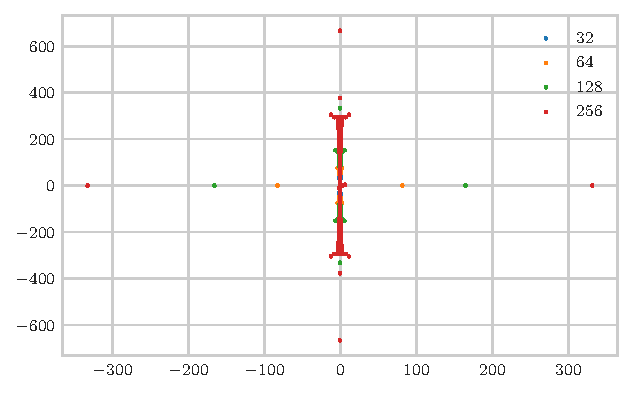
\includegraphics[width=\textwidth]{/home/jeff-severino/SWIRL/CodeRun/03-plotReport/tex-outputs/gam.nonconv.scatter_2nd_order_comp.pdf}
     \caption{Discrete Acoustic Disturbances: Cylinder, Uniform Mean Flow with Liner.}
 \end{figure}
 
 



 \begin{figure}
     \centering
     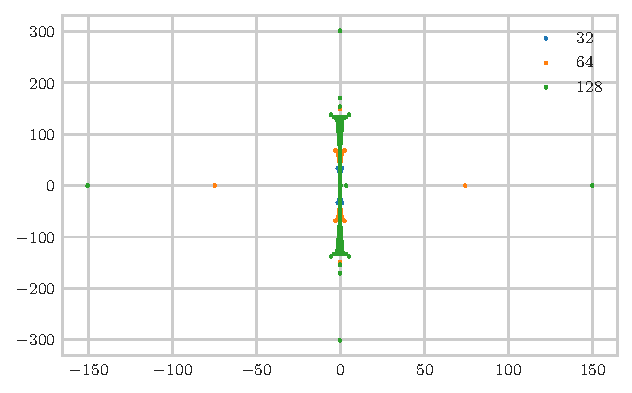
\includegraphics[width=\textwidth]{/home/jeff-severino/SWIRL/CodeRun/03-plotReport/tex-outputs/gam.nonconv.scatter_4th_order_comp.pdf}
     \caption{Discrete Acoustic Disturbances: Cylinder, Uniform Mean Flow with Liner.}
 \end{figure}
 
 


 \begin{figure}
     \centering
     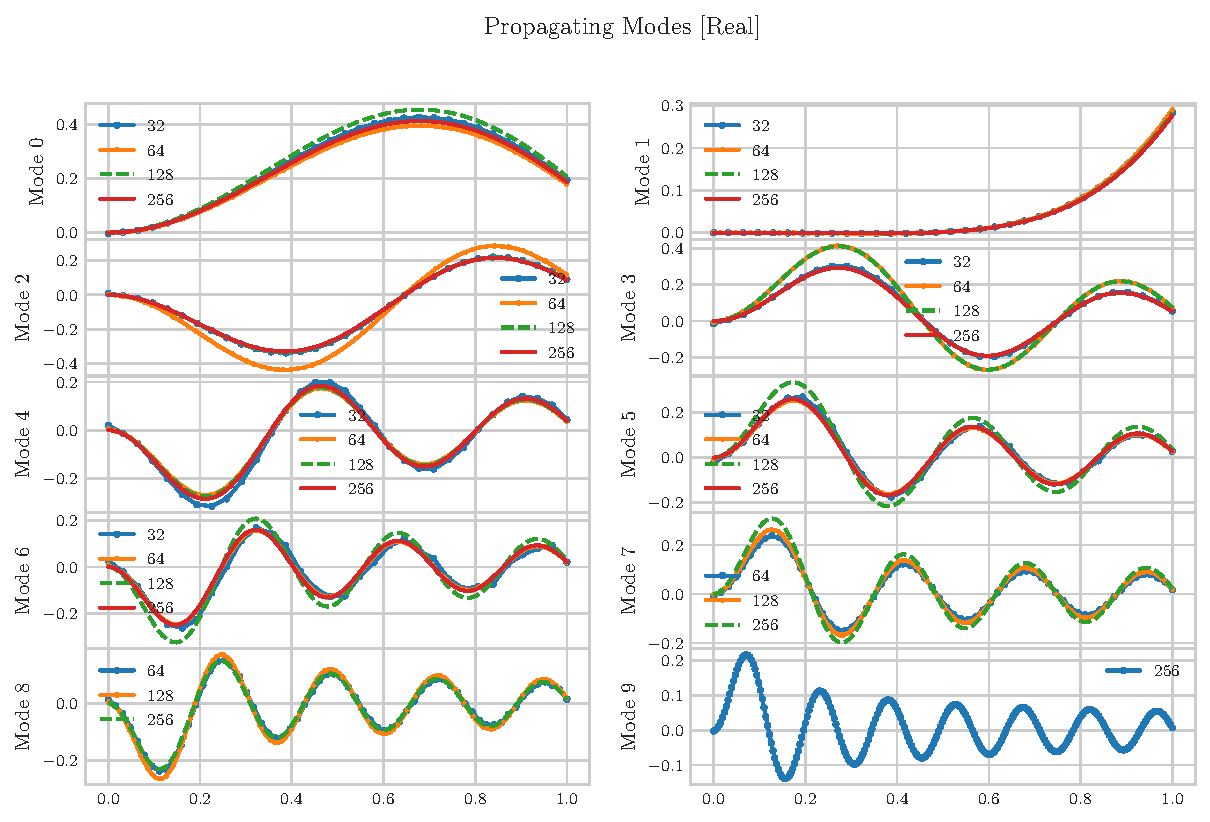
\includegraphics[width=\textwidth]{/home/jeff-severino/SWIRL/CodeRun/03-plotReport/tex-outputs/egv_prop_re.pdf}
 \end{figure}

 \begin{figure}
     \centering
     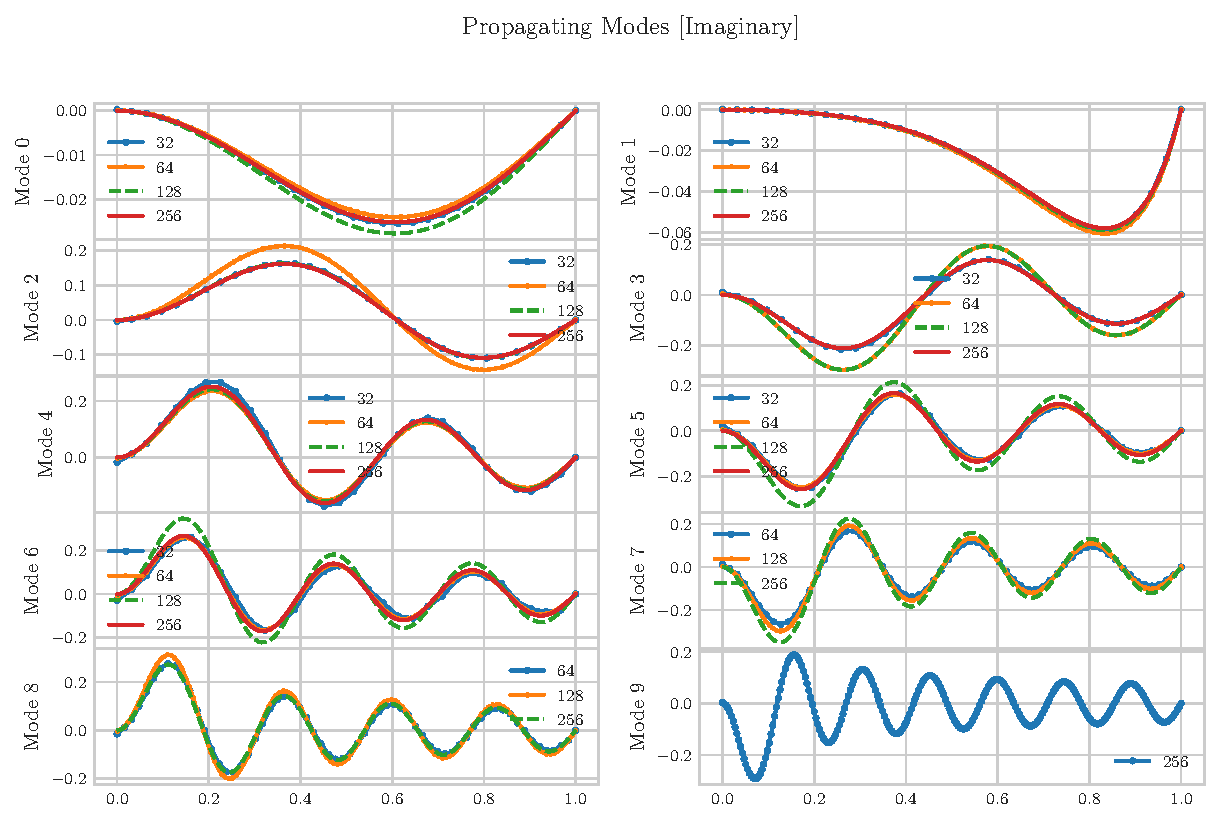
\includegraphics[width=\textwidth]{/home/jeff-severino/SWIRL/CodeRun/03-plotReport/tex-outputs/egv_prop_im.pdf}
 \end{figure}

 \begin{figure}
     \centering
     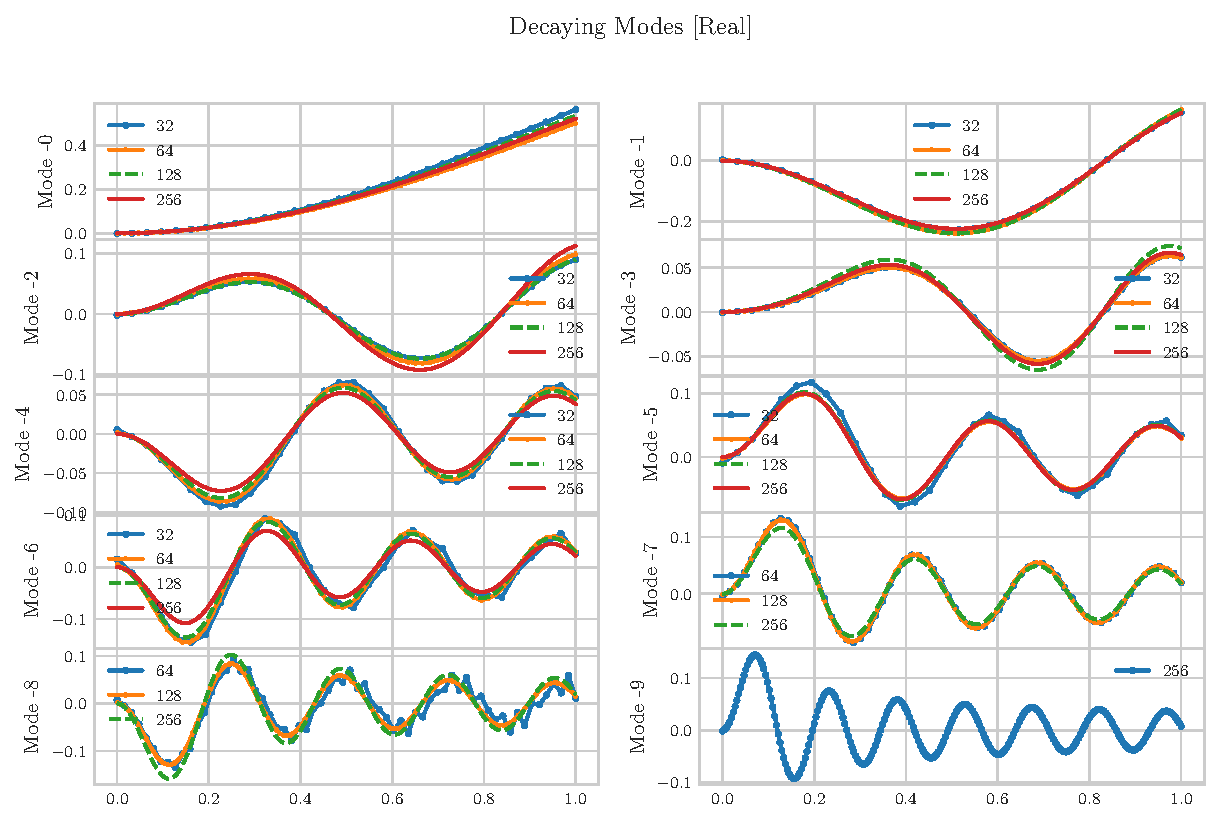
\includegraphics[width=\textwidth]{/home/jeff-severino/SWIRL/CodeRun/03-plotReport/tex-outputs/egv_decay_re.pdf}
 \end{figure}

 \begin{figure}
     \centering
     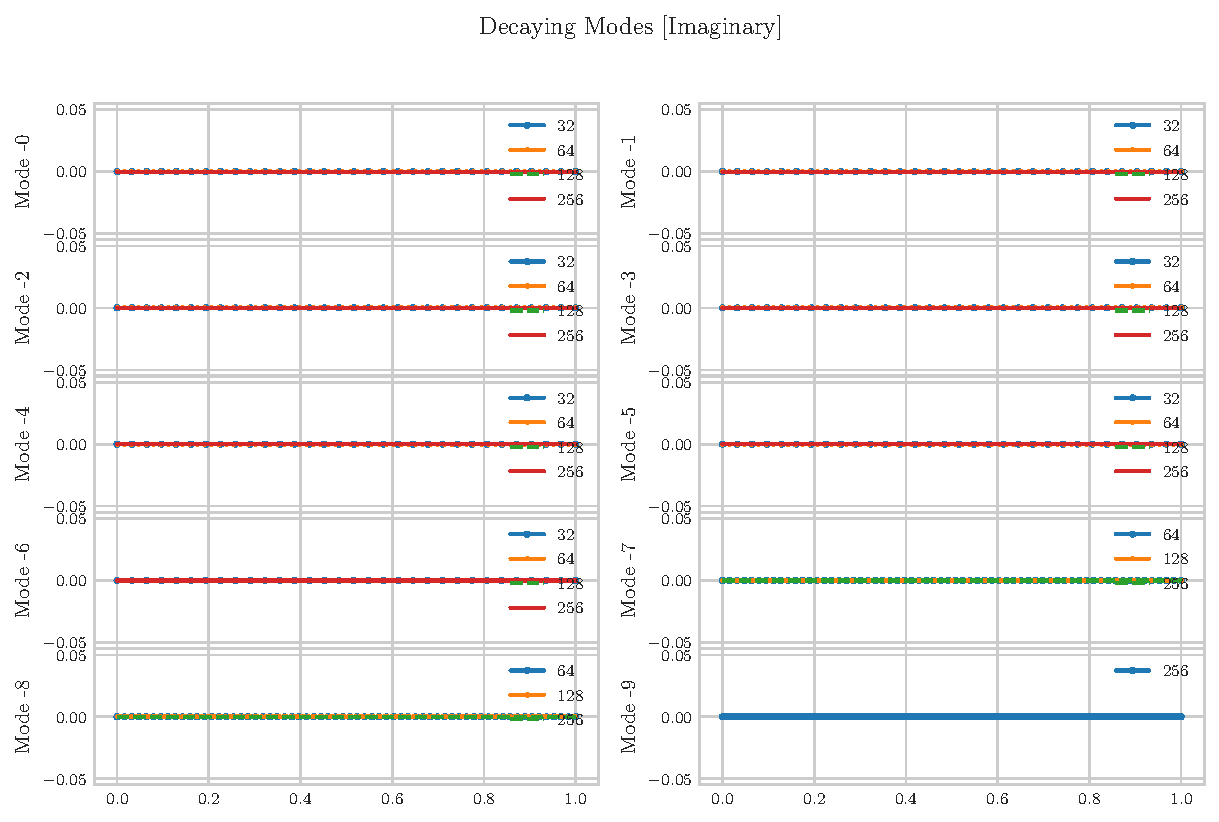
\includegraphics[width=\textwidth]{/home/jeff-severino/SWIRL/CodeRun/03-plotReport/tex-outputs/egv_decay_im.pdf}
 \end{figure}

%  \begin{figure}
%      \centering
%      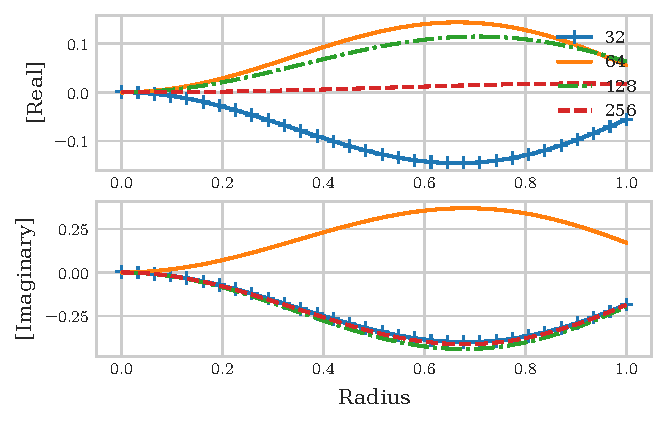
\includegraphics[width=\textwidth]{/home/jeff-severino/SWIRL/CodeRun/03-plotReport/tex-outputs/egv1.pdf}
%      \caption{Propagating Mode $\gamma^+_0 = 0.620-5.014i$}
%  \end{figure}


%  \begin{figure}
%      \centering
%      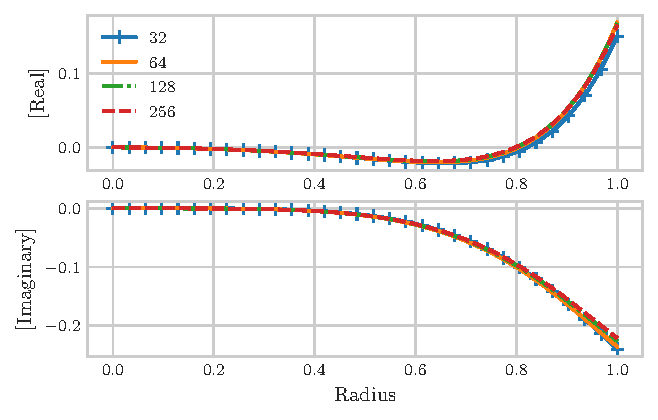
\includegraphics[width=\textwidth]{/home/jeff-severino/SWIRL/CodeRun/03-plotReport/tex-outputs/egv2.pdf}
%      \caption{Propagating Mode $\gamma^+_1 = -5.820-3.897i$}
%  \end{figure}


%  \begin{figure}
%      \centering
%      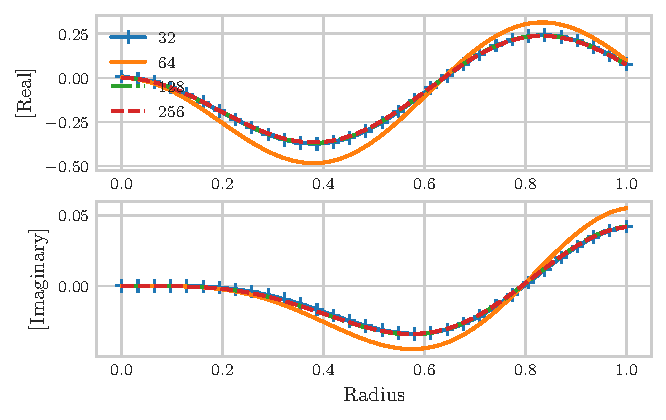
\includegraphics[width=\textwidth]{/home/jeff-severino/SWIRL/CodeRun/03-plotReport/tex-outputs/egv3.pdf}
%      \caption{Propagating Mode $\gamma^+_2 = 0.445-9.187i$}
%  \end{figure}


 % \begin{figure}
 %     \centering
 %     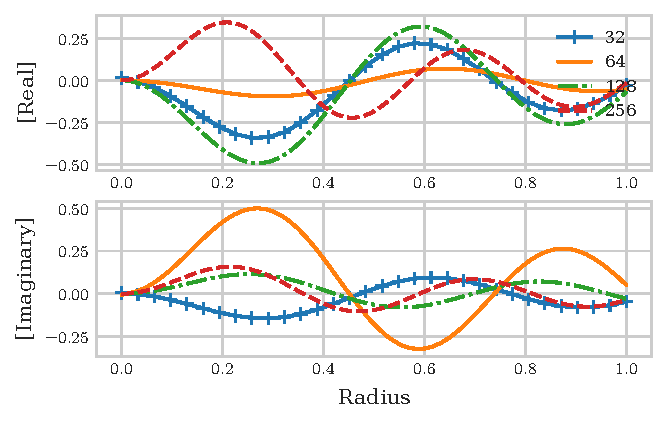
\includegraphics[width=\textwidth]{/home/jeff-severino/SWIRL/CodeRun/03-plotReport/tex-outputs/egv4.pdf}
 %     \caption{Propagating Mode $\gamma^+_3 = 0.453-13.062i$}
 % \end{figure}


 % \begin{figure}
 %     \centering
 %     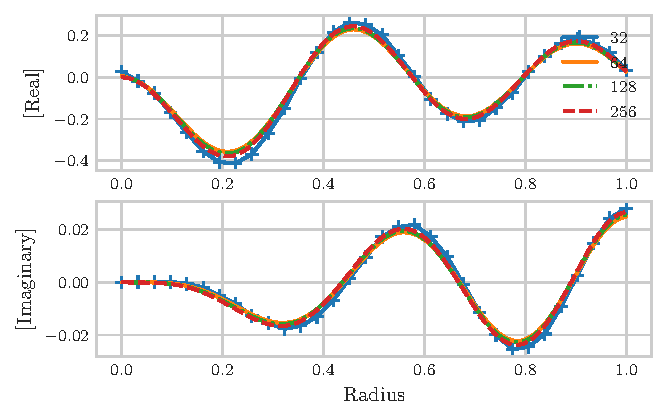
\includegraphics[width=\textwidth]{/home/jeff-severino/SWIRL/CodeRun/03-plotReport/tex-outputs/egv5.pdf}
 %     \caption{Propagating Mode $\gamma^+_4 = 0.480 - 16.822i$}
 % \end{figure}


 % \begin{figure}
 %     \centering
 %     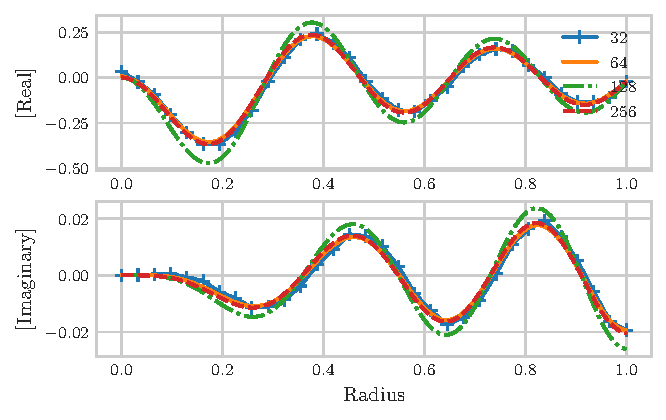
\includegraphics[width=\textwidth]{/home/jeff-severino/SWIRL/CodeRun/03-plotReport/tex-outputs/egv6.pdf}
 %     \caption{Propagating Mode $\gamma^+_5 = 0.503 - 20.531$}
 % \end{figure}


 % \begin{figure}
 %     \centering
 %     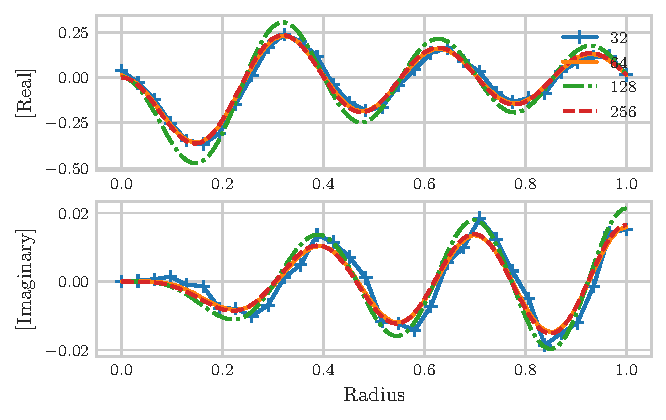
\includegraphics[width=\textwidth]{/home/jeff-severino/SWIRL/CodeRun/03-plotReport/tex-outputs/egv7.pdf}
 %     \caption{Propagating Mode $\gamma^+_6 = 0.522 - 24.213i$}
 % \end{figure}

 % \begin{figure}
 %     \centering
 %     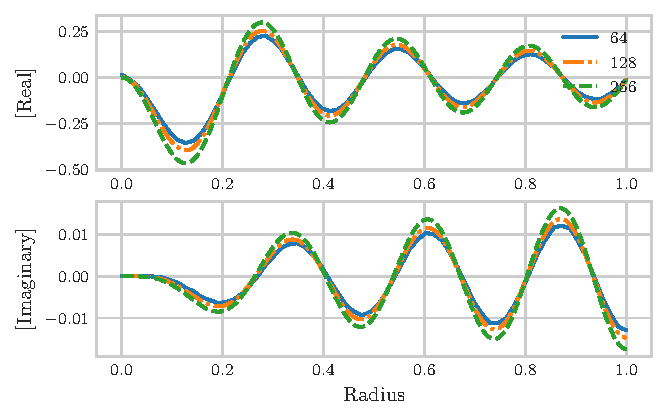
\includegraphics[width=\textwidth]{/home/jeff-severino/SWIRL/CodeRun/03-plotReport/tex-outputs/egv8.pdf}
 %     \caption{Propagating Mode $\gamma^+_7 = 0.538 - 27.880i$}
 % \end{figure}


 % \begin{figure}
 %     \centering
 %     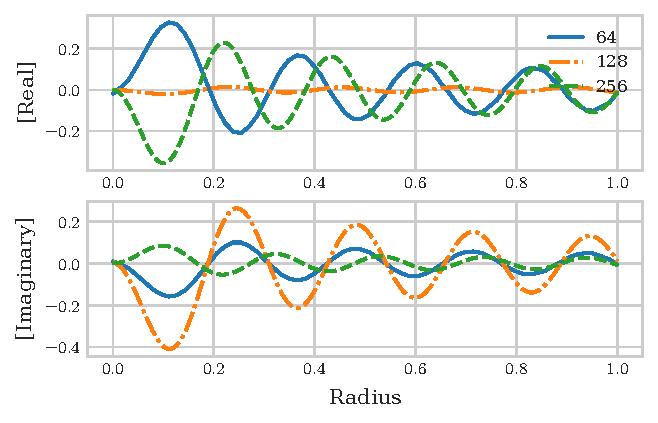
\includegraphics[width=\textwidth]{/home/jeff-severino/SWIRL/CodeRun/03-plotReport/tex-outputs/egv9.pdf}
 %     \caption{Propagating Mode $\gamma^+_8 = 0.550 - 31.537$}
 % \end{figure}




 % \begin{figure}
 %     \centering
 %     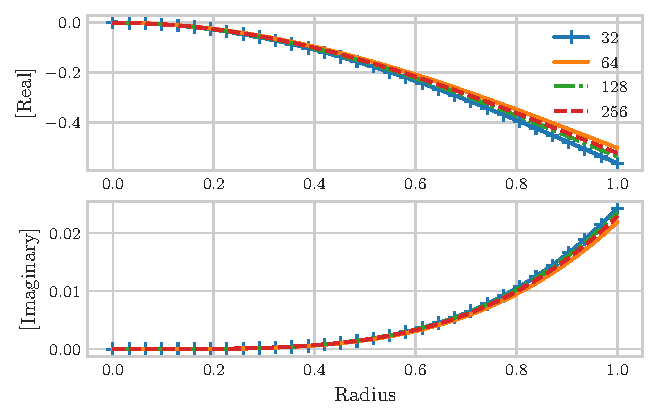
\includegraphics[width=\textwidth]{/home/jeff-severino/SWIRL/CodeRun/03-plotReport/tex-outputs/egv_m1.pdf}
 %     \caption{Propagating Mode $\gamma^-_0 = 0.410-1.290i$}
 % \end{figure}


 % \begin{figure}
 %     \centering
 %     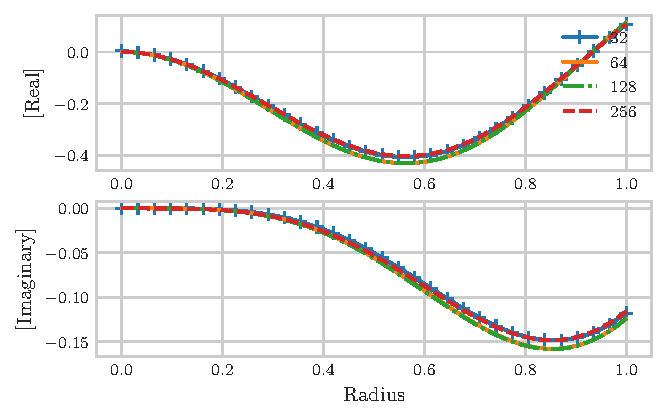
\includegraphics[width=\textwidth]{/home/jeff-severino/SWIRL/CodeRun/03-plotReport/tex-outputs/egv_m2.pdf}
 %     \caption{Propagating Mode $\gamma^-_0 = 0.410-1.290i$}
 % \end{figure}


 % \begin{figure}
 %     \centering
 %     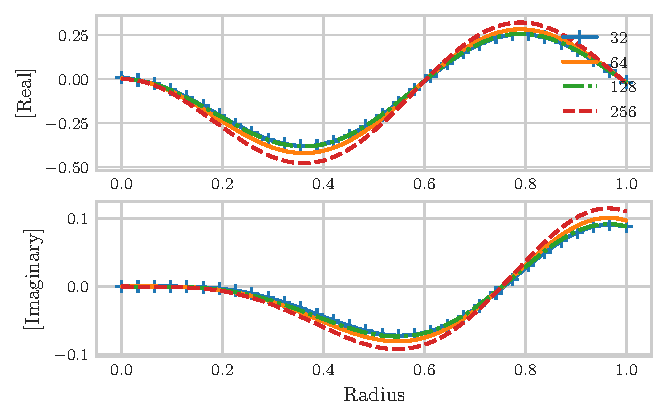
\includegraphics[width=\textwidth]{/home/jeff-severino/SWIRL/CodeRun/03-plotReport/tex-outputs/egv_m3.pdf}
 %     \caption{Propagating Mode $\gamma^-_0 = 0.410-1.290i$}
 % \end{figure}


 % \begin{figure}
 %     \centering
 %     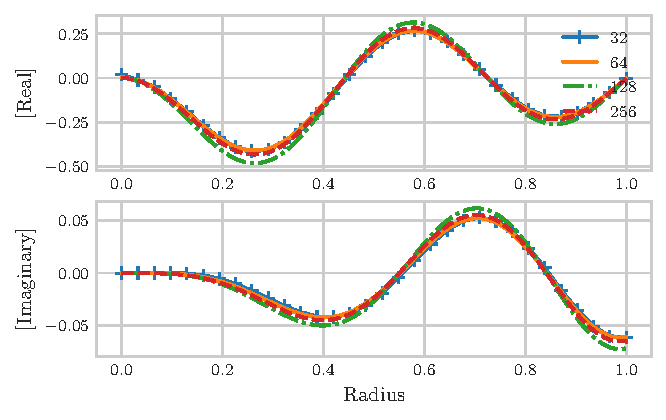
\includegraphics[width=\textwidth]{/home/jeff-severino/SWIRL/CodeRun/03-plotReport/tex-outputs/egv_m4.pdf}
 %     \caption{Propagating Mode $\gamma^-_0 = 0.410-1.290i$}
 % \end{figure}


 % \begin{figure}
 %     \centering
 %     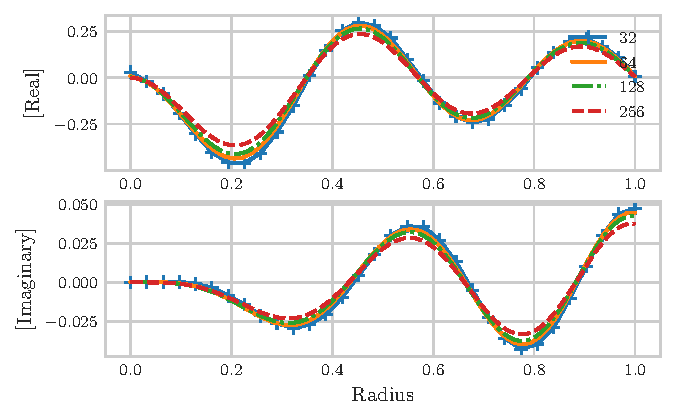
\includegraphics[width=\textwidth]{/home/jeff-severino/SWIRL/CodeRun/03-plotReport/tex-outputs/egv_m5.pdf}
 %     \caption{Propagating Mode $\gamma^-_0 = 0.410-1.290i$}
 % \end{figure}


 % \begin{figure}
 %     \centering
 %     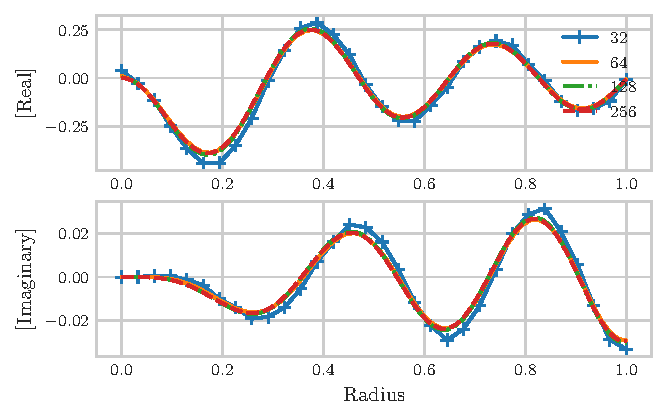
\includegraphics[width=\textwidth]{/home/jeff-severino/SWIRL/CodeRun/03-plotReport/tex-outputs/egv_m6.pdf}
 %     \caption{Propagating Mode $\gamma^-_0 = 0.410-1.290i$}
 % \end{figure}


 % \begin{figure}
 %     \centering
 %     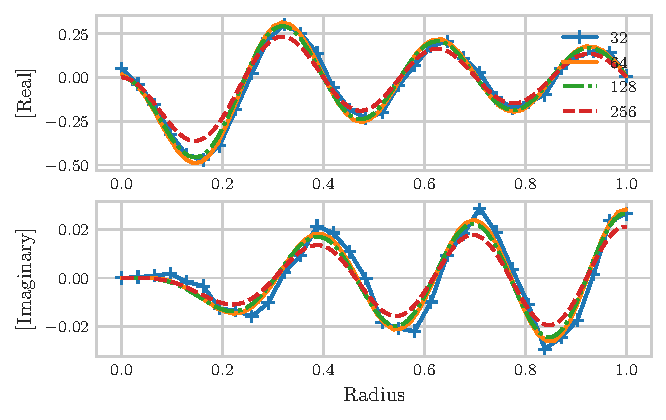
\includegraphics[width=\textwidth]{/home/jeff-severino/SWIRL/CodeRun/03-plotReport/tex-outputs/egv_m7.pdf}
 %     \caption{Propagating Mode $\gamma^-_0 = 0.410-1.290i$}
 % \end{figure}


 % \begin{figure}
 %     \centering
 %     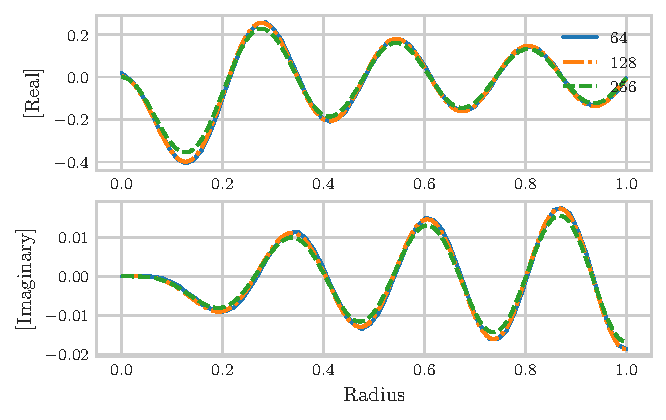
\includegraphics[width=\textwidth]{/home/jeff-severino/SWIRL/CodeRun/03-plotReport/tex-outputs/egv_m8.pdf}
 %     \caption{Propagating Mode $\gamma^-_0 = 0.410-1.290i$}
 % \end{figure}


 % \begin{figure}
 %     \centering
 %     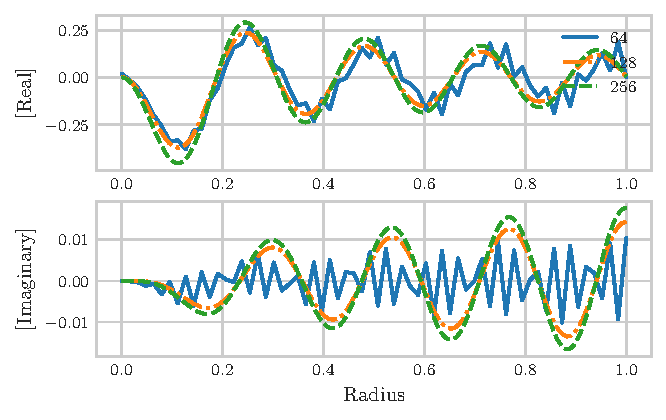
\includegraphics[width=\textwidth]{/home/jeff-severino/SWIRL/CodeRun/03-plotReport/tex-outputs/egv_m9.pdf}
 %     \caption{Propagating Mode $\gamma^-_0 = 0.410-1.290i$}
 % \end{figure}

%  \begin{figure}
%      \centering
%      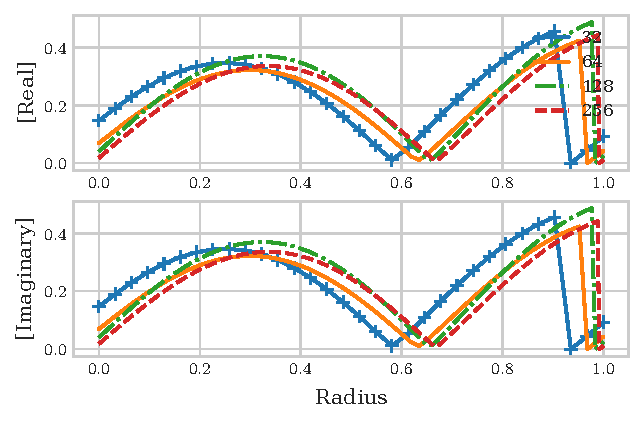
\includegraphics[width=\textwidth]{/home/jeff-severino/SWIRL/CodeRun/03-plotReport/tex-outputs/egvMag1.pdf}
%      \caption{Propagating Mode $\gamma^+_0 = 0.620-5.014i$}
%  \end{figure}


%  \begin{figure}
%      \centering
%      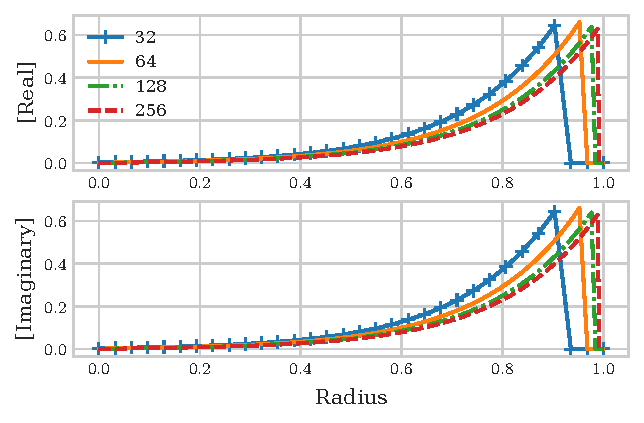
\includegraphics[width=\textwidth]{/home/jeff-severino/SWIRL/CodeRun/03-plotReport/tex-outputs/egvMag2.pdf}
%      \caption{Propagating Mode $\gamma^+_1 = -5.820-3.897i$}
%  \end{figure}


%  \begin{figure}
%      \centering
%      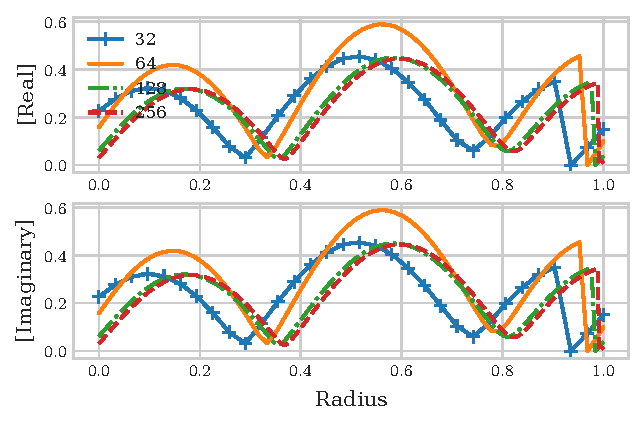
\includegraphics[width=\textwidth]{/home/jeff-severino/SWIRL/CodeRun/03-plotReport/tex-outputs/egvMag3.pdf}
%      \caption{Propagating Mode $\gamma^+_2 = -0.445-9.187i$}
%  \end{figure}


%  \begin{figure}
%      \centering
%      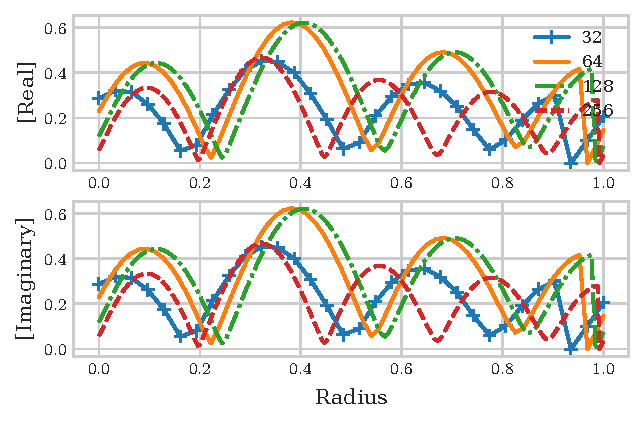
\includegraphics[width=\textwidth]{/home/jeff-severino/SWIRL/CodeRun/03-plotReport/tex-outputs/egvMag4.pdf}
%      \caption{Propagating Mode $\gamma^+_3 = -0.453-13.062i$}
%  \end{figure}


%  \begin{figure}
%      \centering
%      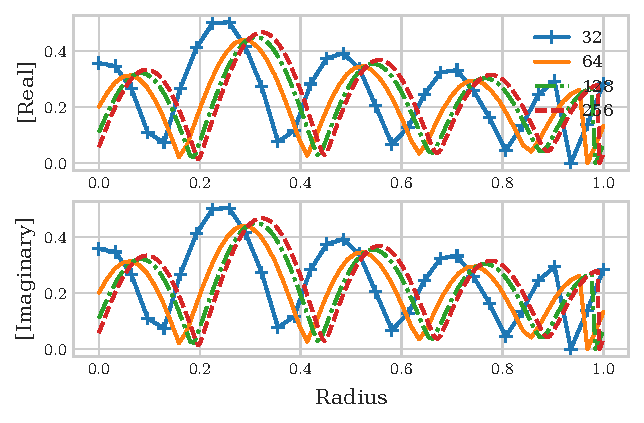
\includegraphics[width=\textwidth]{/home/jeff-severino/SWIRL/CodeRun/03-plotReport/tex-outputs/egvMag5.pdf}
%      \caption{Propagating Mode $\gamma^+_4 = 0.480 - 16.822i$}
%  \end{figure}


%  \begin{figure}
%      \centering
%      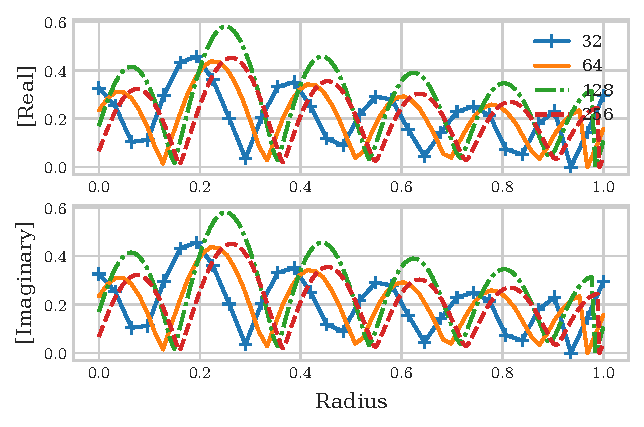
\includegraphics[width=\textwidth]{/home/jeff-severino/SWIRL/CodeRun/03-plotReport/tex-outputs/egvMag6.pdf}
%      \caption{Propagating Mode $\gamma^+_5 = 0.503 - 20.531$}
%  \end{figure}


%  \begin{figure}
%      \centering
%      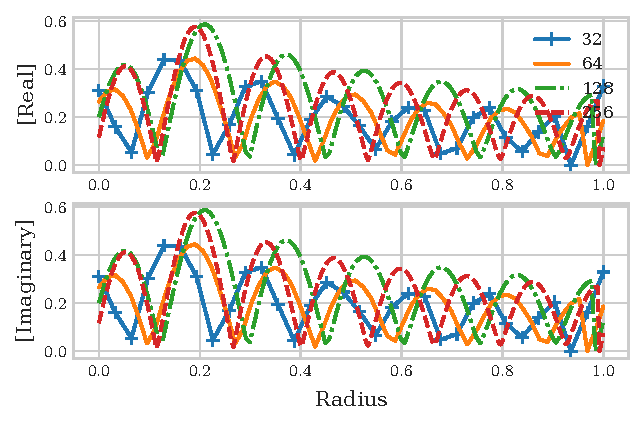
\includegraphics[width=\textwidth]{/home/jeff-severino/SWIRL/CodeRun/03-plotReport/tex-outputs/egvMag7.pdf}
%      \caption{Propagating Mode $\gamma^+_6 = 0.522 - 24.213i$}
%  \end{figure}

%  \begin{figure}
%      \centering
%      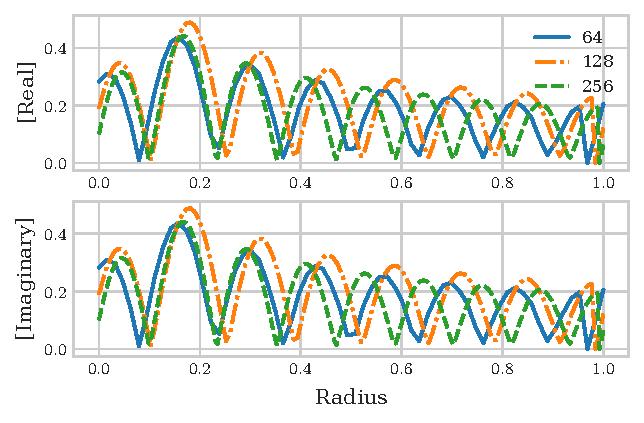
\includegraphics[width=\textwidth]{/home/jeff-severino/SWIRL/CodeRun/03-plotReport/tex-outputs/egvMag8.pdf}
%      \caption{Propagating Mode $\gamma^+_7 = 0.538 - 27.880i$}
%  \end{figure}


%  \begin{figure}
%      \centering
%      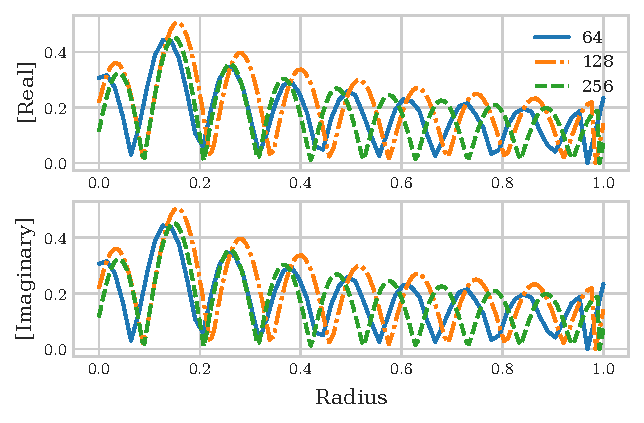
\includegraphics[width=\textwidth]{/home/jeff-severino/SWIRL/CodeRun/03-plotReport/tex-outputs/egvMag9.pdf}
%      \caption{Propagating Mode $\gamma^+_8 = 0.550 - 31.537$}
%  \end{figure}



%  \begin{figure}
%      \centering
%      \includegraphics[width=\textwidth]{/home/jeff-severino/SWIRL/CodeRun/03-plotReport/tex-outputs/egv10.pdf}
%      \caption{Propagating Mode $\gamma^+_8 = 0.550 - 31.537i$}
%  \end{figure}


%  \begin{figure}
%      \centering
%      \includegraphics[width=\textwidth]{/home/jeff-severino/SWIRL/CodeRun/03-plotReport/tex-outputs/egv11.pdf}
%      \caption{Propagating Mode $\gamma^+_9 = 0.589 - 49.75i$}
%  \end{figure}


%  \begin{figure}
%      \centering
%      \includegraphics[width=\textwidth]{/home/jeff-severino/SWIRL/CodeRun/03-plotReport/tex-outputs/egv12.pdf}
%      \caption{Propagating Mode $\gamma^-_0 = 0.410-1.290i$}
%  \end{figure}


%  \begin{figure}
%      \centering
%      \includegraphics[width=\textwidth]{/home/jeff-severino/SWIRL/CodeRun/03-plotReport/tex-outputs/egv13.pdf}
%      \caption{Propagating Mode $\gamma^-_1 = 1.259 + 6.085i$}
%  \end{figure}


%  \begin{figure}
%      \centering
%      \includegraphics[width=\textwidth]{/home/jeff-severino/SWIRL/CodeRun/03-plotReport/tex-outputs/egv14.pdf}
%      \caption{Propagating Mode $\gamma^-_2 = 1.146 + 9.668i$}
%  \end{figure}


%  \begin{figure}
%      \centering
%      \includegraphics[width=\textwidth]{/home/jeff-severino/SWIRL/CodeRun/03-plotReport/tex-outputs/egv15.pdf}
%      \caption{Propagating Mode $\gamma^-_3 = 1.022 + 13.315i$}
%  \end{figure}


%  \begin{figure}
%      \centering
%      \includegraphics[width=\textwidth]{/home/jeff-severino/SWIRL/CodeRun/03-plotReport/tex-outputs/egv16.pdf}
%      \caption{Propagating Mode $\gamma^-_4 = 0.943 + 16.977i$}
%  \end{figure}


%  \begin{figure}
%      \centering
%      \includegraphics[width=\textwidth]{/home/jeff-severino/SWIRL/CodeRun/03-plotReport/tex-outputs/egv17.pdf}
%      \caption{Propagating Mode $\gamma^-_5 = 0.891 +20.635i$}
%  \end{figure}


%  \begin{figure}
%      \centering
%      \includegraphics[width=\textwidth]{/home/jeff-severino/SWIRL/CodeRun/03-plotReport/tex-outputs/egv18.pdf}
%      \caption{Propagating Mode $\gamma^-_6 = 0.855 + 24.288i$}
%  \end{figure}

%  \begin{figure}
%      \centering
%      \includegraphics[width=\textwidth]{/home/jeff-severino/SWIRL/CodeRun/03-plotReport/tex-outputs/egv19.pdf}
%      \caption{Propagating Mode $\gamma^-_7 = 0.829 + 27.937i$}
%  \end{figure}


%  \begin{figure}
%      \centering
%      \includegraphics[width=\textwidth]{/home/jeff-severino/SWIRL/CodeRun/03-plotReport/tex-outputs/egv20.pdf}
%      \caption{Propagating Mode $\gamma^-_8 = 0.809 + 31.581i$}
%  \end{figure}


%  \begin{figure}
%      \centering
%      \includegraphics[width=\textwidth]{/home/jeff-severino/SWIRL/CodeRun/03-plotReport/tex-outputs/egv21.pdf}
%      \caption{Propagating Mode $\gamma^-_9 = 0.755 + 49.77i$}
%  \end{figure}


%  \begin{figure}
%      \centering
%      \includegraphics[width=\textwidth]{/home/jeff-severino/SWIRL/CodeRun/03-plotReport/tex-outputs/egv22.pdf}
%  \end{figure}

%%\begin{tiny}
%    \verbatiminput{../04-EVanalysis/cv.waves.dat}
%\end{tiny}
%
% %\begin{tiny}
% %    \verbatiminput{../04-EVanalysis/gammas0007.dat}
% %\end{tiny}
%% \begin{figure}
%%     \begin{center}
%%         \begin{tikzpicture}[gnuplot]
%% generated with GNUPLOT 5.2p8 (Lua 5.3; terminal rev. Nov 2018, script rev. 108)
%% Tue 21 Sep 2021 04:42:31 PM EDT
\path (0.000,0.000) rectangle (12.500,8.750);
\gpcolor{color=gp lt color axes}
\gpsetlinetype{gp lt axes}
\gpsetdashtype{gp dt axes}
\gpsetlinewidth{0.50}
\draw[gp path] (1.320,0.985)--(11.947,0.985);
\gpcolor{color=gp lt color border}
\gpsetlinetype{gp lt border}
\gpsetdashtype{gp dt solid}
\gpsetlinewidth{1.00}
\draw[gp path] (1.320,0.985)--(1.500,0.985);
\draw[gp path] (11.947,0.985)--(11.767,0.985);
\node[gp node right] at (1.136,0.985) {$0.1$};
\draw[gp path] (1.320,2.107)--(1.410,2.107);
\draw[gp path] (11.947,2.107)--(11.857,2.107);
\draw[gp path] (1.320,2.764)--(1.410,2.764);
\draw[gp path] (11.947,2.764)--(11.857,2.764);
\draw[gp path] (1.320,3.229)--(1.410,3.229);
\draw[gp path] (11.947,3.229)--(11.857,3.229);
\draw[gp path] (1.320,3.591)--(1.410,3.591);
\draw[gp path] (11.947,3.591)--(11.857,3.591);
\draw[gp path] (1.320,3.886)--(1.410,3.886);
\draw[gp path] (11.947,3.886)--(11.857,3.886);
\draw[gp path] (1.320,4.136)--(1.410,4.136);
\draw[gp path] (11.947,4.136)--(11.857,4.136);
\draw[gp path] (1.320,4.352)--(1.410,4.352);
\draw[gp path] (11.947,4.352)--(11.857,4.352);
\draw[gp path] (1.320,4.542)--(1.410,4.542);
\draw[gp path] (11.947,4.542)--(11.857,4.542);
\gpcolor{color=gp lt color axes}
\gpsetlinetype{gp lt axes}
\gpsetdashtype{gp dt axes}
\gpsetlinewidth{0.50}
\draw[gp path] (1.320,4.713)--(11.947,4.713);
\gpcolor{color=gp lt color border}
\gpsetlinetype{gp lt border}
\gpsetdashtype{gp dt solid}
\gpsetlinewidth{1.00}
\draw[gp path] (1.320,4.713)--(1.500,4.713);
\draw[gp path] (11.947,4.713)--(11.767,4.713);
\node[gp node right] at (1.136,4.713) {$1$};
\draw[gp path] (1.320,5.835)--(1.410,5.835);
\draw[gp path] (11.947,5.835)--(11.857,5.835);
\draw[gp path] (1.320,6.492)--(1.410,6.492);
\draw[gp path] (11.947,6.492)--(11.857,6.492);
\draw[gp path] (1.320,6.957)--(1.410,6.957);
\draw[gp path] (11.947,6.957)--(11.857,6.957);
\draw[gp path] (1.320,7.319)--(1.410,7.319);
\draw[gp path] (11.947,7.319)--(11.857,7.319);
\draw[gp path] (1.320,7.614)--(1.410,7.614);
\draw[gp path] (11.947,7.614)--(11.857,7.614);
\draw[gp path] (1.320,7.864)--(1.410,7.864);
\draw[gp path] (11.947,7.864)--(11.857,7.864);
\draw[gp path] (1.320,8.080)--(1.410,8.080);
\draw[gp path] (11.947,8.080)--(11.857,8.080);
\draw[gp path] (1.320,8.270)--(1.410,8.270);
\draw[gp path] (11.947,8.270)--(11.857,8.270);
\gpcolor{color=gp lt color axes}
\gpsetlinetype{gp lt axes}
\gpsetdashtype{gp dt axes}
\gpsetlinewidth{0.50}
\draw[gp path] (1.320,8.441)--(11.947,8.441);
\gpcolor{color=gp lt color border}
\gpsetlinetype{gp lt border}
\gpsetdashtype{gp dt solid}
\gpsetlinewidth{1.00}
\draw[gp path] (1.320,8.441)--(1.500,8.441);
\draw[gp path] (11.947,8.441)--(11.767,8.441);
\node[gp node right] at (1.136,8.441) {$10$};
\gpcolor{color=gp lt color axes}
\gpsetlinetype{gp lt axes}
\gpsetdashtype{gp dt axes}
\gpsetlinewidth{0.50}
\draw[gp path] (1.320,0.985)--(1.320,8.441);
\gpcolor{color=gp lt color border}
\gpsetlinetype{gp lt border}
\gpsetdashtype{gp dt solid}
\gpsetlinewidth{1.00}
\draw[gp path] (1.320,0.985)--(1.320,1.165);
\draw[gp path] (1.320,8.441)--(1.320,8.261);
\node[gp node center] at (1.320,0.677) {$0.5$};
\gpcolor{color=gp lt color axes}
\gpsetlinetype{gp lt axes}
\gpsetdashtype{gp dt axes}
\gpsetlinewidth{0.50}
\draw[gp path] (2.383,0.985)--(2.383,8.441);
\gpcolor{color=gp lt color border}
\gpsetlinetype{gp lt border}
\gpsetdashtype{gp dt solid}
\gpsetlinewidth{1.00}
\draw[gp path] (2.383,0.985)--(2.383,1.165);
\draw[gp path] (2.383,8.441)--(2.383,8.261);
\node[gp node center] at (2.383,0.677) {$0.51$};
\gpcolor{color=gp lt color axes}
\gpsetlinetype{gp lt axes}
\gpsetdashtype{gp dt axes}
\gpsetlinewidth{0.50}
\draw[gp path] (3.445,0.985)--(3.445,8.441);
\gpcolor{color=gp lt color border}
\gpsetlinetype{gp lt border}
\gpsetdashtype{gp dt solid}
\gpsetlinewidth{1.00}
\draw[gp path] (3.445,0.985)--(3.445,1.165);
\draw[gp path] (3.445,8.441)--(3.445,8.261);
\node[gp node center] at (3.445,0.677) {$0.52$};
\gpcolor{color=gp lt color axes}
\gpsetlinetype{gp lt axes}
\gpsetdashtype{gp dt axes}
\gpsetlinewidth{0.50}
\draw[gp path] (4.508,0.985)--(4.508,8.441);
\gpcolor{color=gp lt color border}
\gpsetlinetype{gp lt border}
\gpsetdashtype{gp dt solid}
\gpsetlinewidth{1.00}
\draw[gp path] (4.508,0.985)--(4.508,1.165);
\draw[gp path] (4.508,8.441)--(4.508,8.261);
\node[gp node center] at (4.508,0.677) {$0.53$};
\gpcolor{color=gp lt color axes}
\gpsetlinetype{gp lt axes}
\gpsetdashtype{gp dt axes}
\gpsetlinewidth{0.50}
\draw[gp path] (5.571,0.985)--(5.571,8.441);
\gpcolor{color=gp lt color border}
\gpsetlinetype{gp lt border}
\gpsetdashtype{gp dt solid}
\gpsetlinewidth{1.00}
\draw[gp path] (5.571,0.985)--(5.571,1.165);
\draw[gp path] (5.571,8.441)--(5.571,8.261);
\node[gp node center] at (5.571,0.677) {$0.54$};
\gpcolor{color=gp lt color axes}
\gpsetlinetype{gp lt axes}
\gpsetdashtype{gp dt axes}
\gpsetlinewidth{0.50}
\draw[gp path] (6.634,0.985)--(6.634,8.441);
\gpcolor{color=gp lt color border}
\gpsetlinetype{gp lt border}
\gpsetdashtype{gp dt solid}
\gpsetlinewidth{1.00}
\draw[gp path] (6.634,0.985)--(6.634,1.165);
\draw[gp path] (6.634,8.441)--(6.634,8.261);
\node[gp node center] at (6.634,0.677) {$0.55$};
\gpcolor{color=gp lt color axes}
\gpsetlinetype{gp lt axes}
\gpsetdashtype{gp dt axes}
\gpsetlinewidth{0.50}
\draw[gp path] (7.696,0.985)--(7.696,8.441);
\gpcolor{color=gp lt color border}
\gpsetlinetype{gp lt border}
\gpsetdashtype{gp dt solid}
\gpsetlinewidth{1.00}
\draw[gp path] (7.696,0.985)--(7.696,1.165);
\draw[gp path] (7.696,8.441)--(7.696,8.261);
\node[gp node center] at (7.696,0.677) {$0.56$};
\gpcolor{color=gp lt color axes}
\gpsetlinetype{gp lt axes}
\gpsetdashtype{gp dt axes}
\gpsetlinewidth{0.50}
\draw[gp path] (8.759,0.985)--(8.759,8.441);
\gpcolor{color=gp lt color border}
\gpsetlinetype{gp lt border}
\gpsetdashtype{gp dt solid}
\gpsetlinewidth{1.00}
\draw[gp path] (8.759,0.985)--(8.759,1.165);
\draw[gp path] (8.759,8.441)--(8.759,8.261);
\node[gp node center] at (8.759,0.677) {$0.57$};
\gpcolor{color=gp lt color axes}
\gpsetlinetype{gp lt axes}
\gpsetdashtype{gp dt axes}
\gpsetlinewidth{0.50}
\draw[gp path] (9.822,0.985)--(9.822,8.441);
\gpcolor{color=gp lt color border}
\gpsetlinetype{gp lt border}
\gpsetdashtype{gp dt solid}
\gpsetlinewidth{1.00}
\draw[gp path] (9.822,0.985)--(9.822,1.165);
\draw[gp path] (9.822,8.441)--(9.822,8.261);
\node[gp node center] at (9.822,0.677) {$0.58$};
\gpcolor{color=gp lt color axes}
\gpsetlinetype{gp lt axes}
\gpsetdashtype{gp dt axes}
\gpsetlinewidth{0.50}
\draw[gp path] (10.884,0.985)--(10.884,7.953);
\draw[gp path] (10.884,8.261)--(10.884,8.441);
\gpcolor{color=gp lt color border}
\gpsetlinetype{gp lt border}
\gpsetdashtype{gp dt solid}
\gpsetlinewidth{1.00}
\draw[gp path] (10.884,0.985)--(10.884,1.165);
\draw[gp path] (10.884,8.441)--(10.884,8.261);
\node[gp node center] at (10.884,0.677) {$0.59$};
\gpcolor{color=gp lt color axes}
\gpsetlinetype{gp lt axes}
\gpsetdashtype{gp dt axes}
\gpsetlinewidth{0.50}
\draw[gp path] (11.947,0.985)--(11.947,8.441);
\gpcolor{color=gp lt color border}
\gpsetlinetype{gp lt border}
\gpsetdashtype{gp dt solid}
\gpsetlinewidth{1.00}
\draw[gp path] (11.947,0.985)--(11.947,1.165);
\draw[gp path] (11.947,8.441)--(11.947,8.261);
\node[gp node center] at (11.947,0.677) {$0.6$};
\draw[gp path] (1.320,8.441)--(1.320,0.985)--(11.947,0.985)--(11.947,8.441)--cycle;
\node[gp node center,rotate=-270] at (0.292,4.713) {Observed Order-of-Accuracy};
\node[gp node center] at (6.633,0.215) {$\Delta $};
\node[gp node right] at (10.479,8.107) {?};
\gpcolor{rgb color={0.000,0.502,0.502}}
\draw[gp path] (10.663,8.107)--(11.579,8.107);
\draw[gp path] (11.947,2.953)--(7.224,3.734)--(4.445,5.212)--(2.930,6.020)--(2.137,6.034)%
  --(1.732,5.886)--(1.527,5.842)--(1.423,5.836)--(1.372,5.835);
\gpsetpointsize{4.00}
\gppoint{gp mark 1}{(11.947,2.953)}
\gppoint{gp mark 1}{(7.224,3.734)}
\gppoint{gp mark 1}{(4.445,5.212)}
\gppoint{gp mark 1}{(2.930,6.020)}
\gppoint{gp mark 1}{(2.137,6.034)}
\gppoint{gp mark 1}{(1.732,5.886)}
\gppoint{gp mark 1}{(1.527,5.842)}
\gppoint{gp mark 1}{(1.423,5.836)}
\gppoint{gp mark 1}{(1.372,5.835)}
\gppoint{gp mark 1}{(11.121,8.107)}
\gpcolor{color=gp lt color border}
\draw[gp path] (1.320,8.441)--(1.320,0.985)--(11.947,0.985)--(11.947,8.441)--cycle;
%% coordinates of the plot area
\gpdefrectangularnode{gp plot 1}{\pgfpoint{1.320cm}{0.985cm}}{\pgfpoint{11.947cm}{8.441cm}}
\end{tikzpicture}
%% gnuplot variables

%%     \end{center}
%%     \caption{Absolute Value Rate of Convergence for the Source Term}
%% \end{figure}
%
\end{document}

